\chapter{Pola wektorowe, przepływy i pochodna Liego}
\label{ch:pola}
\index{pole wektorowe}

W Rozdziale~\ref{ch:rozmaitosci} zbudowaliśmy przestrzenie styczne i wiązkę $TM$.
Teraz wybieramy wektor \emph{w każdym} punkcie, w sposób gładki.
Otrzymujemy pole wektorowe: jednocześnie operator
różniczkowy, kierunek ruchu i infinitezymalny generator lokalnych dyfeomorfizmów.
Z tego jednego pojęcia wynikają nawias Liego, krzywe całkowe, przepływy oraz
pochodna Liego.

Rozdział rozwija rachunek pól oraz geometrię ich przepływów: najpierw
rozwiązujemy równanie krzywej całkowej, a następnie badamy ruch
punktów i sposób przenoszenia funkcji oraz pól wektorowych.
Do dalszej topologii różniczkowej przydadzą się zwłaszcza prostowanie
pola, pola zależne od czasu oraz rozszerzanie izotopii.
Przez $M$ rozumiemy rozmaitość gładką w sensie Definicji~\ref{def:rozmaitosc-gladka},
bez brzegu, chyba że wyraźnie zaznaczono inaczej.
Wszystkie pola i odwzorowania są klasy $C^\infty$.
Uwagi o brzegu i końcach przedziału czasu rozumiemy
według Definicji~\ref{def:rozmaitosc-z-brzegiem-1}
i opisu przestrzeni stycznej w
Stwierdzeniu~\ref{prop:styczna-brzeg-1}.
Tak samo interpretujemy gładkie rodziny na domkniętym przedziale czasu.



\section{Pola wektorowe i derywacje globalne}
\label{sec:derywacje}

W Sekcji~\ref{sec:przestrzen-styczna} utożsamiliśmy wektor $v\in T_pM$ z
\emph{derywacją w punkcie} $v\colon C^\infty(M)\to\R$:
po zastosowaniu do funkcji otrzymujemy liczbę. Pole wybiera taki
wektor w każdym punkcie, a jego działanie na funkcję zwraca nową
funkcję. Rozróżnienie tych dwóch typów derywacji będzie istotne.

\begin{definicja}
\emph{Pole wektorowe} $X$ na $M$ to gładka sekcja wiązki stycznej
$TM\to M$, czyli gładkie odwzorowanie $X\colon M\to TM$ spełniające
$X(p)\in T_pM$ dla każdego $p$. Przestrzeń pól oznaczamy $\X(M)=\Gamma(TM)$.
\end{definicja}

Wartość pola w ustalonym punkcie oznaczamy $X_p:=X(p)$.
Jest to jeden wektor styczny w $T_pM$; zapis $X_p(f)$ oznacza
działanie tego wektora jako derywacji w punkcie $p$ na funkcję $f$.
Na przykład wzór $X_{(u,v)}=(-v,u)$ na $\R^2$, po utożsamieniu
$T_{(u,v)}\R^2$ z $\R^2$, określa pole:
w każdym punkcie przypisuje wektor styczny zależny gładko od $(u,v)$.
Poza początkiem układu wektor jest styczny do okręgu o środku w zerze,
a w początku $X_{(0,0)}=0$.

W mapie $(U;x^1,\ldots,x^n)$ pole zapisuje się jednoznacznie jako
\begin{equation}\label{eq:lokalne-pole}
 X\big|_U=\sum_{i=1}^{n}X^i\frac{\partial}{\partial x^i},
 \qquad X^i\in C^\infty(U).
\end{equation}
Dokładniej, dla $p\in U$ jest to równość w $T_pM$:
$X_p=\sum_iX^i(p)\,\partial_{x^i}|_p$.
Lokalna trywializacja $TM$ z Rozdziału~\ref{ch:rozmaitosci}
pokazuje, że gładkość sekcji $X$ jest równoważna gładkości
wszystkich $X^i$ w każdej mapie. W drugą stronę gładkie współczynniki
na obszarach map określają jedno pole, jeżeli na przecięciach
opisują te same wektory styczne.

Geometrycznie $X_p$ wskazuje kierunek i prędkość w punkcie $p$.
Jeżeli $f\in C^\infty(M)$, czyli $f\colon M\to\R$,
opisuje na przykład temperaturę, to $X_p(f)$ jest chwilowym
tempem jej zmiany w kierunku wyznaczonym przez $X_p$.

Sprawdźmy tę interpretację na krzywej reprezentującej $X_p$.
W modelu z Sekcji~\ref{sec:przestrzen-styczna} każdy wektor
styczny jest reprezentowany przez klasę krzywych.
Wybierzmy mapę $(U,\varphi)$ wokół $p$, gdzie
$\varphi=(x^1,\ldots,x^n)$, i zapiszmy
$X_p=\sum_{i=1}^n X^i(p)\,\partial_{x^i}|_p$.
Na $\varphi(U)$ używamy standardowych współrzędnych
$u^1,\ldots,u^n$.
Oznaczmy $a=(X^1(p),\ldots,X^n(p))\in\R^n$ i rozważmy
krzywą $c(t)=\varphi(p)+ta$ w przestrzeni współrzędnych.
Ponieważ $\varphi(U)$ jest otwarty i $c(0)=\varphi(p)$,
istnieje $\varepsilon>0$ takie, że
$c((-\varepsilon,\varepsilon))\subset\varphi(U)$.
Możemy zatem zdefiniować
\[
\gamma\colon(-\varepsilon,\varepsilon)\to U,
\qquad
\gamma(t)=\varphi^{-1}\bigl(\varphi(p)+ta\bigr).
\]
Krzywa ta jest gładka i spełnia $\gamma(0)=p$ oraz
$(\varphi\circ\gamma)'(0)=a$, więc jej klasa $[\gamma]$
odpowiada wektorowi $X_p$ przy utożsamieniu
z rozdziału~1.

Pokażemy, że $X_p(f)$ jest pochodną funkcji $f$
wzdłuż skonstruowanej krzywej. Ponieważ
$\gamma=\varphi^{-1}\circ c$ i $\gamma(t)\in U$,
złożenie $f\circ\gamma$ jest dobrze określone oraz
$f\circ\gamma=(f\circ\varphi^{-1})\circ c$.
Stosując regułę łańcucha, otrzymujemy
\[
\begin{aligned}
\left.\frac{\dd}{\dd t}\right|_{t=0}f(\gamma(t))
&=D(f\circ\varphi^{-1})(\varphi(p))\cdot c'(0)\\
&=\sum_{i=1}^n X^i(p)
  \frac{\partial(f\circ\varphi^{-1})}{\partial u^i}
  (\varphi(p))
=X_p(f).
\end{aligned}
\]
Ostatnia równość wynika z definicji derywacji
współrzędnościowych. Rachunek obowiązuje dla każdej krzywej
o klasie $[\gamma]=X_p$: jej prędkość w mapie w chwili $t=0$
jest zawsze równa $a$. Niezależność tej klasy od wyboru mapy
ustaliliśmy w Sekcji~\ref{sec:przestrzen-styczna}.

Krzywa $\gamma$ reprezentuje zatem wektor w jednym
punkcie; jej dalszy przebieg nie wpływa na $X_p(f)$.
Nie musi być przy tym krzywą całkową pola $X$,
gdyż wymagamy jedynie zgodności jej wektora stycznego
z $X_p$ w chwili $t=0$.


\begin{definicja}
\emph{Derywacją} algebry $C^\infty(M)$ nazywamy $\R$-liniowe odwzorowanie
$D\colon C^\infty(M)\to C^\infty(M)$ spełniające regułę Leibniza
\[
 D(fg)=fD(g)+gD(f),\qquad f,g\in C^\infty(M).
\]
Zbiór takich derywacji oznaczamy $\operatorname{Der}_{\R}(C^\infty(M))$.
\end{definicja}

Warunek $\R$-liniowości oznacza liniowość względem stałych liczb.
Z reguły Leibniza wynika $D(1)=D(1\cdot1)=2D(1)$, więc $D(1)=0$
i $D(c)=0$ dla stałej $c$. Derywacja nie jest na ogół
$C^\infty(M)$-liniowa jako operator na funkcjach: jej działanie na
$hf$ zawiera dodatkowy składnik $fD(h)$.

Zacznijmy od pola $X$. Dla każdej funkcji $f\in C^\infty(M)$ określamy
\emph{funkcję} $D_X(f)$ przez
\[
 D_X(f)(p):=X_p(f),\qquad p\in M.
\]
W mapie $X_p=\sum_iX^i(p)\,\partial_i|_p$, więc
\[
 D_X(f)\big|_U=\sum_i X^i\partial_i f,
 \qquad D_X(f)(p)=\sum_iX^i(p)\,\partial_i f(p).
\]
W pierwszym wzorze $\partial_i f$ oznacza lokalną pochodną
$f\circ\varphi^{-1}$, przeniesioną z powrotem na $U$.
Suma gładkich funkcji jest gładka. Drugi wzór daje liczbę, bo
po ustaleniu $p$ współczynniki $X^i(p)$ są liczbami.
Punktowa reguła Leibniza dla $X_p$ daje
$D_X(fg)=fD_X(g)+gD_X(f)$ po sprawdzeniu równości w każdym punkcie.
Tak z pola otrzymujemy derywację globalną $D_X$.

W drugą stronę zacznijmy od \emph{dowolnej} derywacji globalnej $D$.
Dla ustalonego $p$ składamy ją z ewaluacją w $p$ i oznaczamy
\[
 v_p(f):=\bigl(D(f)\bigr)(p),\qquad
 C^\infty(M)\xrightarrow{\ D\ }C^\infty(M)
 \xrightarrow{\ \operatorname{ev}_p\ }\R.
\]
Funkcjonał $v_p$ jest $\R$-liniowy. Po ewaluacji globalnej
reguły Leibniza dostajemy \emph{punktową} regułę:
\[
 v_p(fg)=f(p)v_p(g)+g(p)v_p(f).
\]
Z definicji przestrzeni stycznej $v_p\in T_pM$; nie jest to już
operator o wartościach funkcyjnych. Lemat~\ref{lem:lokalnosc}
zapewnia, że $v_p(f)=D(f)(p)$ zależy tylko od kiełka $f$ w $p$.
Samo złożenie z ewaluacją daje na razie rodzinę wektorów;
jej gładkość trzeba jeszcze udowodnić.

\begin{twierdzenie}\label{thm:derywacje-pola}
Odwzorowanie
\[
 \X(M)\longrightarrow\operatorname{Der}_{\R}(C^\infty(M)),
 \qquad X\longmapsto D_X,\qquad D_X(f)(p)=X_p(f),
\]
jest izomorfizmem $C^\infty(M)$-modułów.
\end{twierdzenie}
\begin{proof}
Sprawdziliśmy wyżej, że $D_X$ jest derywacją, a dowolna
derywacja globalna $D$ wyznacza wektory $X_p(f):=D(f)(p)$.
Pozostaje pokazać, że $X\colon p\mapsto X_p$ jest gładką sekcją.

Ustalmy $p_0\in M$ i mapę $(U;x^1,\ldots,x^n)$ wokół $p_0$.
Wybierzmy otoczenie $V$ punktu $p_0$ o zwartym domknięciu zawartym w $U$
oraz funkcję odcinającą $\chi\in C^\infty(M)$, równą $1$ na
otoczeniu $\overline V$ i o nośniku zawartym w $U$.
Funkcja $\widetilde x^i$, zadana na $U$ przez $\chi x^i$ i równa
$0$ poza $U$, jest gładka na $M$. Na $V$ ma ten sam kiełek co $x^i$.
Z Twierdzenia~\ref{tw:baza-styczna} (po ewentualnym przesunięciu
początku współrzędnych) i lokalności derywacji punktowych
wynika, że dla $p\in V$
\[
 X_p=\sum_i a^i(p)\,\frac{\partial}{\partial x^i}\Big|_p,
 \qquad a^i(p)=X_p(\widetilde x^i)=D(\widetilde x^i)(p).
\]
Istotnie, działanie obu stron na $\widetilde x^j$ daje tę samą
liczbę $a^j(p)$, ponieważ
$\partial_{x^i}|_p(\widetilde x^j)=\delta_i^j$.
Każde $a^i=D(\widetilde x^i)|_V$ jest gładkie, gdyż $D$ przyjmuje
wartości w $C^\infty(M)$. Gładkość lokalnych współczynników
wokół każdego $p_0$ dowodzi gładkości $X$.

Dla każdego $f$ i $p$ mamy z konstrukcji
$D_X(f)(p)=X_p(f)=D(f)(p)$, zatem $D_X=D$.
Odwrotnie, jeśli zaczniemy od pola $X$, to ewaluacja $D_X$
w $p$ odzyskuje $X_p$ jako derywację punktową. Konstrukcje są więc
wzajemnie odwrotne. Dodawanie pól odpowiada dodawaniu derywacji,
a dla $h\in C^\infty(M)$ zachodzi
$D_{hX}(f)(p)=h(p)X_p(f)=(hD_X)(f)(p)$.
\end{proof}

Odtąd skracamy zapis $D_X(f)$ do $X(f)$; jest to funkcja na $M$,
podczas gdy $X_p(f)=X(f)(p)$ jest liczbą.

Na przykład na $\R$ operator $D(f)(x)=x^2f'(x)$ jest derywacją
globalną: $D(fg)(x)=x^2(f'(x)g(x)+f(x)g'(x))
=D(f)(x)g(x)+f(x)D(g)(x)$. Odpowiada mu pole
$X=x^2\partial_x$. W ustalonym punkcie $p$ jego wektor
$X_p=p^2\,\frac{\dd}{\dd x}\big|_p$ działa na funkcję przez
$X_p(f)=p^2f'(p)$; w szczególności $X_2(f)=4f'(2)$.
Współczynnik $x^2$ pola staje się liczbą $p^2$ po ustaleniu punktu.

\begin{uwaga}[Moduł pól i lokalne bazy]
Przestrzeń $\X(M)$ jest modułem nad pierścieniem funkcji:
$(hX)_p=h(p)X_p$. Po stronie derywacji mnożenie określa wzór
$(hD)(f)=hD(f)$; reguła Leibniza dla $hD$ wynika przez pomnożenie
obu stron reguły dla $D$ przez $h$.
Nie musi istnieć globalna baza modułu $\X(M)$ nad $C^\infty(M)$.
Na przykład $TS^2$ nie jest wiązką trywialną; nie da się wybrać
dwóch globalnych, wszędzie liniowo niezależnych pól na sferze.
Lokalne bazy $\partial_{x^1},\ldots,\partial_{x^n}$ zawsze istnieją.
Używamy tu klasycznego twierdzenia o nieistnieniu nigdzie
niezerowego pola na $S^2$; wynika ono również z późniejszego
Twierdzenia~\ref{thm:poincare-hopf-16} i $\chi(S^2)=2$.
\end{uwaga}

\begin{uwaga}[Przeniesienie pola przez mapę i zmiana współrzędnych]
Niech $(U,\varphi)$ będzie mapą rozmaitości $M$
o współrzędnych $x^1,\ldots,x^n$.
Ponieważ $\varphi\colon U\to\varphi(U)$ jest dyfeomorfizmem,
przenosi pole $X$ z $U$ na otwarty zbiór $\varphi(U)\subset\R^n$:
\begin{equation}\label{eq:pole-przeniesione-mapa}
\widehat X_\varphi(u)
:=(\dd\varphi)_{\varphi^{-1}(u)}X_{\varphi^{-1}(u)},
\qquad u\in\varphi(U).
\end{equation}
Piszemy $X_\varphi^i$ dla współczynników $X^i$
ze wzoru~\eqref{eq:lokalne-pole} w tej mapie;
indeks $\varphi$ odróżnia je od współczynników w innej mapie.
Jeśli $p=\varphi^{-1}(u)$ i
$X_p=\sum_iX_\varphi^i(p)\,\partial_{x^i}|_p$,
to współczynniki $\widehat X_\varphi(u)$ w standardowej bazie
$T_u\R^n$ wynoszą $X_\varphi^i(p)$.

W drugiej mapie $(V,\psi)$, o współrzędnych $y^1,\ldots,y^n$,
to samo pole ma na $U\cap V$ zapis
$X=\sum_jX_\psi^j\partial_{y^j}$.
Oznaczmy $G=\psi\circ\varphi^{-1}$.
Z reguły łańcucha dla $\psi=G\circ\varphi$ dostajemy
\[
\widehat X_\psi\bigl(G(u)\bigr)
=DG(u)\,\widehat X_\varphi(u),
\qquad u\in\varphi(U\cap V).
\]
Porównując $j$-te składowe, otrzymujemy regułę zmiany
współczynników pola:
\begin{equation}\label{eq:transformacja-wspolczynnikow-pola}
X_\psi^j(p)=\sum_i\frac{\partial y^j}{\partial x^i}(p)\,X_\varphi^i(p).
\end{equation}
Jest to ten sam rachunek co zmiana baz
z~\eqref{eq:transformacja-derywacji}.
Na przykład dla zmiany współrzędnej $y=2x$ na $\R$ pole
$X=a(x)\partial_x$ ma w nowej współrzędnej postać
$X=2a(y/2)\partial_y$.
\end{uwaga}

\begin{uwaga}[Od pola w przestrzeni otaczającej do współrzędnych]
Prześledźmy kolejność kroków, którą zastosujemy na okręgu i sferze.
Niech $M\subset\R^N$ będzie gładką podrozmaitością zanurzoną,
z inkluzją
$\iota\colon M\hookrightarrow\R^N$. Najpierw znamy pole $W$
na $\R^N$. Sprawdzamy, czy w punktach $p\in M$ jego wektor
$W_p\in T_p\R^N$ jest styczny do $M$, czyli należy do obrazu
$(\dd\iota)_p(T_pM)$. Dopiero wtedy możemy mówić o polu na samej
rozmaitości: ponieważ $(\dd\iota)_p$ jest injektywna
(Stwierdzenie~\ref{stw:styczna-podrozmaitosci}), istnieje
jedyny $X_p\in T_pM$ taki, że
\[
(\dd\iota)_pX_p=W_p.
\]
To są wektory w dwóch różnych przestrzeniach stycznych;
nie stosujemy $(\dd\varphi)_p$ bezpośrednio do $W_p$.
Gładkość $X$ wynika z gładkości $W$: w lokalnej parametryzacji
różniczka inkluzji ma rząd $\dim M$, więc współczynniki $X$
otrzymujemy lokalnie z gładkiego układu liniowego o nieosobliwym minorze.

Teraz wybieramy mapę $\varphi\colon U\to D\subset\R^n$ i piszemy
$u=\varphi(p)$. Korzystając ze wzoru~\eqref{eq:pole-przeniesione-mapa},
zapisujemy pole przeniesione na obszar współrzędnych $D$ jako
\[
\widehat X_\varphi(u)
=\sum_{i=1}^n a^i(u)\,
  \frac{\partial}{\partial u^i}\Big|_u,
\qquad a^i(u):=X_\varphi^i(\varphi^{-1}(u)).
\]
Liczby $a^i(u)=X_\varphi^i(p)$ są poszukiwanymi współczynnikami.
Wcześniejsza zmiana map porównywała dwa opisy \emph{tego samego}
pola $X$; tutaj przed użyciem mapy otrzymaliśmy $X$ z pola
otaczającego $W$. Jeśli $X$ jest już dane na $M$, zaczynamy
od wyboru mapy.

Dlaczego w rachunku pojawia się $\varphi^{-1}$? Aby porównać
nieznane współczynniki z danym wektorem $W_p$, wracamy z $D$
na $M$ przez $(\dd\varphi^{-1})_u$, a potem przechodzimy
do $\R^N$ przez $(\dd\iota)_p$. Równość
$(\dd\varphi^{-1})_u\widehat X_\varphi(u)=X_p$ wynika
z~$\varphi^{-1}\circ\varphi=\mathrm{id}_U$. Dla
$F=\iota\circ\varphi^{-1}\colon D\to\R^N$ reguła łańcucha daje
schemat w przestrzeniach stycznych:
\[
T_uD\ \xrightarrow{\ (\dd\varphi^{-1})_u\ }\ T_pM
\ \xrightarrow{\ (\dd\iota)_p\ }\ T_p\R^N,
\qquad
W_{F(u)}=(\dd F)_u\widehat X_\varphi(u)
=\sum_{i=1}^n a^i(u)\frac{\partial F}{\partial u^i}(u).
\]
Różniczka $\varphi^{-1}$ pokazuje więc, jak wektor zapisany
współrzędnymi wygląda na $M$; różniczka $F$ pokazuje ten sam
wektor w przestrzeni otaczającej. Ostatnie równanie pozwala
obliczyć $a^i(u)$ z podanego $W_p$ przez porównanie składowych.
\end{uwaga}

\begin{przyklad}[Pole obrotowe na okręgu]
Okrąg $S_r^1=\{(u,v)\in\R^2:u^2+v^2=r^2\}$, $r>0$,
jest jednowymiarową rozmaitością. Zanurzamy go w płaszczyźnie
przez inkluzję $\iota\colon S_r^1\hookrightarrow\R^2$,
$\iota(u,v)=(u,v)$; dla $r=1$ jest to zwykłe $S^1$.
Rozważmy na $\R^2$ pole
$W=-v\partial_u+u\partial_v$. Dla $p=(u,v)\in S_r^1$ mamy
$p\cdot W_p=-uv+vu=0$. Ponieważ przestrzeń styczna okręgu,
oglądana przez $(\dd\iota)_p$, jest prostopadła do $p$
(Stwierdzenie~\ref{stw:styczna-normalne-euklidesowe}),
$W_p$ jest styczny do okręgu. Dostajemy zatem jednoznaczne
pole $X$ na $S_r^1$ określone przez $(\dd\iota)_pX_p=W_p$.

Wybierzmy teraz otwarty przedział $I$ długości mniejszej niż $2\pi$.
Odwzorowanie $\gamma\colon I\to S_r^1$,
$\gamma(t)=(r\cos t,r\sin t)$, opisuje otwarty łuk
$U=\gamma(I)$ i jest odwrotnością lokalnej mapy kątowej
$\varphi\colon U\to I$. Po złożeniu z inkluzją otrzymujemy
parametryzację w płaszczyźnie
$F=\iota\circ\varphi^{-1}=\iota\circ\gamma\colon I\to\R^2$;
ma ona ten sam wzór $F(t)=(r\cos t,r\sin t)$.
Oznaczmy $p=\gamma(t)$. Na tym łuku zapis pola na rozmaitości
ma postać $X_p=a(t)\,\partial_t|_p$, gdzie
$a(t)=X_\varphi^1(\varphi^{-1}(t))$.
Chcemy znaleźć liczbę $a(t)$.
Zgodnie ze schematem przenosimy $X_p$ do $T_tI$ przez
$(\dd\varphi)_p$; otrzymujemy
$\widehat X_\varphi(t)=a(t)\,\partial_t|_t$.
Znamy jednak wektor $W_p$ w płaszczyźnie, więc porównamy oba
wektory po przeniesieniu z powrotem przez $(\dd F)_t$.
Reguła łańcucha daje
\[
\begin{aligned}
(\dd F)_t\!\left(\frac{\partial}{\partial t}\Big|_t\right)
&=\frac{\dd F}{\dd t}(t)
=(-r\sin t,r\cos t)\\
&=W_p.
\end{aligned}
\]
Ponieważ $(\dd F)_t=(\dd\iota)_p\circ(\dd\varphi^{-1})_t$,
różniczka odwrotności mapy przenosi $\partial_t|_t$ na wektor
bazy $\partial_t|_p$ na okręgu, a różniczka inkluzji pokazuje
go jako $(-r\sin t,r\cos t)$ w $T_p\R^2$.
Teraz
\[
W_p=(\dd F)_t\widehat X_\varphi(t)
=a(t)(-r\sin t,r\cos t).
\]
Pochodna $F'(t)$ jest niezerowa dla $r>0$, więc $a(t)=1$.
Równoważnie $X_p=\partial_t|_p$ i
$\widehat X_\varphi(t)=\partial_t|_t$. Wektor
$(-r\sin t,r\cos t)$ zapisujemy w bazie
$\partial_u|_p,\partial_v|_p$ przestrzeni $T_p\R^2$;
pojedynczy $\partial_u|_p$ na ogół nie jest styczny do okręgu.

Sprawdźmy teraz działanie pola na funkcje. Dla $g(u,v)=u$
otrzymujemy zmienną wzdłuż okręgu funkcję
$g\circ\gamma(t)=r\cos t$, a więc
$X(g|_{S_r^1})(\gamma(t))=\frac{\dd}{\dd t}(r\cos t)=-r\sin t$.
Natomiast dla $f(u,v)=u^2+v^2$ bierzemy
$h=f|_{S_r^1}$. Wzór współrzędnościowy daje
\[
X(h)\bigl(\gamma(t)\bigr)
=a(t)\frac{\dd}{\dd t}(h\circ\gamma)(t)
=\frac{\dd}{\dd t}\bigl(r^2\cos^2t+r^2\sin^2t\bigr)=0.
\]
Ta sama konstrukcja mapy działa lokalnie wokół każdego punktu okręgu.
Wynik $X(h)=0$ pokazuje, że pole nie zmienia wartości $f$ na
okręgu, zgodnie ze stycznością do poziomicy $f^{-1}(r^2)=S_r^1$.
Samo pole jest niezerowe, co widać z $F'(t)\ne0$.
\end{przyklad}

\begin{przyklad}[Pole na sferze]
Niech $S^2=\{(x,y,z)\in\R^3:x^2+y^2+z^2=1\}$.
Jak na okręgu, zaczynamy od pola w przestrzeni otaczającej:
$W=-y\partial_x+x\partial_y$ na $\R^3$, bez składowej
w kierunku $z$. Niech $\iota\colon S^2\hookrightarrow\R^3$
będzie inkluzją. W punkcie $p=(x,y,z)\in S^2$ wektor pola
otaczającego ma postać $W_p=(-y,x,0)$. Ponieważ
$p\cdot W_p=-xy+xy=0$, a obraz $(\dd\iota)_p(T_pS^2)$
jest płaszczyzną prostopadłą do $p$
(Stwierdzenie~\ref{stw:styczna-normalne-euklidesowe}),
$W_p$ jest styczny
do sfery. Określa zatem jednoznaczne gładkie pole $X$ na
$S^2$ przez $(\dd\iota)_pX_p=W_p$. Wzór na $W$ podaje
więc pole na całej sferze, zanim wybierzemy jakąkolwiek mapę.

Chcemy teraz odczytać współczynniki $X$ w jednej mapie.
Niech $U=\{(x,y,z)\in S^2:z>0\}$ będzie górną półsferą,
$D=\{(u,v)\in\R^2:u^2+v^2<1\}$, a
$\varphi\colon U\to D$ mapą $\varphi(x,y,z)=(x,y)=(u,v)$.
Współrzędne $x,y,z$ w $\R^3$ nie są trzema niezależnymi
współrzędnymi na $S^2$: wiąże je równanie $x^2+y^2+z^2=1$.
Na $U$ wystarczą dwie współrzędne $u,v$, gdyż
$z=\sqrt{1-u^2-v^2}>0$. W punkcie
$p=\varphi^{-1}(u,v)$ zapiszmy więc
$X_p=a(u,v)\,\partial_u|_p+b(u,v)\,\partial_v|_p$.
Po utożsamieniu $T_{(u,v)}D$ z $\R^2$ jego obraz ma postać
$\widehat X_\varphi(u,v)=(a(u,v),b(u,v))$.
Szukamy tych dwóch liczb.

Wiemy, jak wygląda $W_p$ w $\R^3$, więc znów wracamy ze
współrzędnych do przestrzeni otaczającej. Odwrotność mapy
razem z inkluzją daje parametryzację
\[
F=\iota\circ\varphi^{-1},\qquad
F(u,v)=(u,v,z(u,v)),\qquad
z(u,v)=\sqrt{1-u^2-v^2}.
\]
Różniczka $\varphi^{-1}$ przenosi wektory bazy z $D$
na wektory styczne do sfery, a $(\dd\iota)_p$ pokazuje je
w $\R^3$. Z reguły łańcucha
$(\dd F)_{(u,v)}=(\dd\iota)_p\circ(\dd\varphi^{-1})_{(u,v)}$.
Ponieważ $\partial_u z=-u/z$ i $\partial_v z=-v/z$,
\[
\dd F_{(u,v)}(a,b)
=a\left(1,0,-\frac{u}{z}\right)
 +b\left(0,1,-\frac{v}{z}\right)
=\left(a,b,-\frac{ua+vb}{z}\right).
\]
Teraz rozwiązujemy równanie ze schematu
$(\dd F)_{(u,v)}(a,b)=W_p=(-v,u,0)$.
Z pierwszych dwóch składowych dostajemy $a=-v$ i $b=u$;
trzecia też się zgadza, bo $u(-v)+vu=0$.
Stąd $X|_U=-v\,\partial_u+u\,\partial_v$.
Otrzymaliśmy ten sam wynik, który dałoby zastosowanie
$(\dd\varphi)_p$ do \emph{wektora stycznego $X_p$ na sferze}:
różniczka mapy bierze z jego obrazu w $\R^3$ pierwsze
dwie składowe. Nie stosujemy jej do pola $W$ zdefiniowanego
na całej $\R^3$.

Pole ma zera na biegunach; poza nimi wskazuje kierunek obrotu
wokół osi $z$. Na Rysunku~\ref{fig:pole-obrotowe-na-sferze}
wyróżniono punkt $p=(0,-\sqrt3/2,1/2)\in U$.
W naszej mapie $(u,v)=(0,-\sqrt3/2)$, więc
$X_p=(\sqrt3/2)\,\partial_u|_p$, a jego obraz w $\R^3$ to
$(\dd\iota)_pX_p=W_p=(\sqrt3/2,0,0)$.
\end{przyklad}

\begin{figure}[H]
\centering
\begin{tikzpicture}[>=Stealth,scale=1.12,line cap=round,line join=round]
% Rzut ortogonalny P(x,y,z)=(x,(y+\sqrt{15}z)/4), ze skalą 1.7.
\shade[inner color=white,outer color=manifoldblue!43] (0,0) circle (1.7);
\coordinate (N) at (0,{1.7*sqrt(15)/4});
\coordinate (S) at (0,{-1.7*sqrt(15)/4});
\draw[manifoldblue!38,densely dashed,thin] (N)--(S);
% Tylna i przednia połowa równika.
\draw[manifoldblue!52,densely dashed,thin]
  (1.7,0) arc[start angle=0,end angle=180,x radius=1.7,y radius=.425];
\draw[manifoldblue!65!black,thin]
  (-1.7,0) arc[start angle=180,end angle=360,x radius=1.7,y radius=.425];
% Widoczny łuk równoleżnika z=1/2.
\draw[manifoldblue!60,thin]
  ({1.7*sqrt(3)/2*cos(225)},
   {1.7*sqrt(15)/8+1.7*sqrt(3)/8*sin(225)})
  arc[start angle=225,end angle=315,
      x radius={1.7*sqrt(3)/2},y radius={1.7*sqrt(3)/8}];
% Wektory są rzutami W_p=(-y,x,0), ze wspólną skalą długości.
\coordinate (pL) at ({1.7*cos(225)},{.425*sin(225)});
\coordinate (pE) at (0,-.425);
\coordinate (pR) at ({1.7*cos(315)},{.425*sin(315)});
\coordinate (p) at (0,{1.7*(sqrt(15)-sqrt(3))/8});
\fill[manifoldred] (pL) circle (1.8pt);
\fill[manifoldred] (pR) circle (1.8pt);
\fill[manifoldred] (pE) circle (1.8pt);
\draw[->,very thick,manifoldred] (pL)
  -- ++({.32*1.7/sqrt(2)},{-.32*.425/sqrt(2)});
\draw[->,very thick,manifoldred] (pR)
  -- ++({.32*1.7/sqrt(2)},{.32*.425/sqrt(2)});
\draw[->,very thick,manifoldred] (pE)
  -- ++(.544,0);
\draw[->,very thick,manifoldred] (p)
  -- ++({.32*1.7*sqrt(3)/2},0)
  node[above right=2pt,font=\small] {$W_p$};
\draw[manifoldblue!75!black,very thick] (0,0) circle (1.7);
\fill[manifoldred] (p) circle (2.2pt)
  node[above left=3pt,font=\small] {$p$};
\fill[manifoldgold!85!black] (N) circle (2.4pt)
  node[above right=2pt,font=\small] {$N$};
\draw[manifoldgold!85!black,densely dashed,thick] (S) circle (2.4pt)
  node[below right=3pt,font=\small] {$S$};
\end{tikzpicture}
\caption{Pole $X$ na sferze, oglądane przez $W_p=(-y,x,0)$ w $\R^3$.
Strzałki są styczne do
równoleżników i wskazują obrót wokół osi $z$. Bieguny $N$ i $S$
są zerami pola; przerywana obwódka oznacza zasłonięty biegun $S$.}
\label{fig:pole-obrotowe-na-sferze}
\end{figure}

\begin{uwaga}[Dwa sposoby obliczania pochodnej funkcji]
Gdy znamy współczynniki pola w mapie, obliczamy $X(f)(p)$
ze wzoru $X=\sum_iX^i\partial_{x^i}$, tak jak na okręgu.
Jeśli $M$ jest gładką podrozmaitością zanurzoną w $\R^N$,
możemy zamiast tego wybrać lokalne gładkie przedłużenie
$\widetilde f$ funkcji $f$ z $M$ do otoczenia $p$ w $\R^N$.
Takie przedłużenie istnieje: w lokalnym modelu, w którym $M$
jest zadana przez zerowe współrzędne normalne, nadajemy
$\widetilde f$ tę samą wartość niezależnie od tych współrzędnych.
Wtedy
$X_p(f)=W_p\cdot\nabla\widetilde f(p)$, gdzie
$(\dd\iota)_pX_p=W_p$: liczymy pochodną $\widetilde f$
wzdłuż krzywej w $M$ o wektorze stycznym $X_p$.
Wynik nie zależy od przedłużenia:
różnica dwóch przedłużeń znika na $M$, więc jej pochodna
wzdłuż każdej krzywej na $M$ jest równa zeru.
\end{uwaga}

\begin{uwaga}[Pole wzdłuż odwzorowania]
Dla gładkiego $F\colon M\to N$ i $X\in\X(M)$ wektory
$\dd F_p(X_p)$ leżą w przestrzeniach $T_{F(p)}N$.
Tworzą \emph{pole wzdłuż $F$}, czyli gładką sekcję wiązki cofniętej
\[
 F^*TN=\{(p,v):p\in M,\ v\in T_{F(p)}N\}\longrightarrow M,
 \qquad(p,v)\longmapsto p.
\]
Jeśli $x^i$ i $y^a$ są odpowiednio współrzędnymi na $M$ i $N$,
to współrzędne tego przekroju nad $p$ mają postać
$\sum_i X^i(p)\,\partial_i(y^a\circ F)(p)$.
Są gładkie, bo $X^i$ i $y^a\circ F$ są gładkie.
Pole wzdłuż $F$ ma za punkt bazowy $p\in M$, nawet gdy dwa różne
punkty $M$ mają ten sam obraz w $N$. Aby pochodziło od pola $Y$ na $N$,
musielibyśmy mieć
\[
 Y_{F(p)}=\dd F_p(X_p)\qquad\text{dla każdego }p\in M.
\]
Wektory po prawej stronie muszą zatem być równe przy wszystkich
przeciwobrazach jednego punktu.

Weźmy $M=N=\R$ oraz $X=\partial_t$ i oznaczmy współrzędną celu przez $y$.
Dla $F(t)=t^2$ reguła łańcucha daje
$\dd F_t(X_t)=2t\,\partial_y|_{t^2}$.
Jeśli $t>0$, punkty $t$ i $-t$ mają ten sam obraz $y=t^2$, więc
postulowane pole $Y$ musiałoby jednocześnie spełniać
\[
 Y_y=2t\,\partial_y|_y
 \qquad\text{oraz}\qquad
 Y_y=-2t\,\partial_y|_y.
\]
To niemożliwe, bo $t\ne0$. Nie otrzymujemy nawet jednoznacznego
przypisania wektora punktom obrazu $F$.

Dla $F(t)=t^3$ każdy $y\in\R$ ma dokładnie jeden przeciwobraz
$t=\sqrt[3]{y}$, więc nie ma już sprzeczności między przeciwobrazami.
Jedynym możliwym polem $Y$ byłoby jednak
\[
 \dd F_t(X_t)=3t^2\,\partial_y|_{t^3},
 \qquad
 Y_y=3|y|^{2/3}\,\partial_y|_y.
\]
Funkcja $a(y)=3|y|^{2/3}$ jest ciągła, lecz w zerze jej iloraz
różnicowy ma postać
\[
 \frac{a(h)-a(0)}{h}
 =3\,\operatorname{sgn}(h)|h|^{-1/3}\qquad(h\ne0),
\]
która nie ma skończonej granicy przy $h\to0$.
Nie istnieje więc gładkie pole $Y$ spełniające podany warunek.
Obie przeszkody dotyczą pary $(F,X)$: dla $F(t)=t^2$ i innego pola
$X=t\partial_t$ otrzymalibyśmy na przykład gładkie
$Y=2y\partial_y$ na $\R$.
Gdy $F$ jest dyfeomorfizmem, otrzymujemy natomiast pole
\[
 (F_*X)_q=\dd F_{F^{-1}(q)}X_{F^{-1}(q)}.
\]
Jest ono gładkie jako złożenie gładkich odwzorowań.
W szczególności $\varphi_*(X|_U)=\widehat X_\varphi$
ze wzoru~\eqref{eq:pole-przeniesione-mapa}.
Natomiast przyporządkowanie
$p\longmapsto(\dd\iota)_pX_p=W_p$ z obu przykładów
jest polem \emph{wzdłuż} inkluzji $\iota$;
wektory $W_p$ leżą w przestrzeniach stycznych do $\R^N$.
\end{uwaga}

\section{Nawias Liego: mierzenie nieprzemienności}
\label{sec:nawias}

Dwa pola są operatorami na funkcjach. Można je więc składać i wziąć
ich komutator.
\begin{definicja}
\emph{Nawiasem Liego} pól $X,Y\in\X(M)$ nazywamy pole $[X,Y]$ zadane przez
\begin{equation}\label{eq:nawias-def}
 [X,Y](f)=X(Y(f))-Y(X(f)),\qquad f\in C^\infty(M).
\end{equation}
\end{definicja}

Choć $X\circ Y$ jako operator jest na ogół drugiego rzędu, wyrazy z
pochodnymi drugimi znoszą się w różnicy.
\begin{fakt}\label{fakt:nawias-wlasnosci}
$[X,Y]$ jest polem wektorowym. Ponadto nawias jest dwuliniowy nad $\R$,
antysymetryczny i spełnia tożsamość Jacobiego
\[
 [X,[Y,Z]]+[Y,[Z,X]]+[Z,[X,Y]]=0.
\]
Jego reguła Leibniza względem funkcji ma postać
\begin{equation}\label{eq:nawias-leibniz}
 [X,fY]=f[X,Y]+X(f)Y,\qquad [fX,Y]=f[X,Y]-Y(f)X.
\end{equation}
\end{fakt}
\begin{proof}
Pokażmy najpierw, że komutator jest derywacją, choć samo
złożenie dwóch derywacji nią zazwyczaj nie jest.
Dla funkcji $f,g$ dwukrotnie stosujemy regułę Leibniza:
\begin{align*}
[X,Y](fg)
&=X\bigl(Y(f)g+fY(g)\bigr)
  -Y\bigl(X(f)g+fX(g)\bigr)\\
&=X(Yf)g+Y(f)X(g)+X(f)Y(g)+fX(Yg)\\
&\quad-Y(Xf)g-X(f)Y(g)-Y(f)X(g)-fY(Xg)\\
&=[X,Y](f)g+f[X,Y](g).
\end{align*}
Wyrazy mieszane znoszą się dokładnie parami. Komutator
jest liniowy nad $\R$ i spełnia regułę Leibniza,
więc z Twierdzenia~\ref{thm:derywacje-pola} odpowiada
gładkiemu polu wektorowemu. Z definicji natychmiast
$[X,Y]=-[Y,X]$; liniowość w obu argumentach wynika
z liniowości składania operatorów.

Sprawdźmy tożsamość Jacobiego, pokazując wszystkie
wyrazy. Jako operatory na funkcjach mamy
\begin{align*}
[X,[Y,Z]]&=XYZ-XZY-YZX+ZYX,\\
[Y,[Z,X]]&=YZX-YXZ-ZXY+XZY,\\
[Z,[X,Y]]&=ZXY-ZYX-XYZ+YXZ.
\end{align*}
Suma prawych stron jest zerowa: np.\ $XYZ$ znosi się
z $-XYZ$, a analogicznie pozostałe pięć możliwych
kolejności. Ponieważ równość operatorów zachodzi na
każdej funkcji, zachodzi równość pól wektorowych.

Na koniec stosujemy definicję do dowolnej funkcji $g$:
\begin{align*}
[X,fY](g)
 &=X\bigl(fY(g)\bigr)-fY\bigl(X(g)\bigr)
  =X(f)Y(g)+f[X,Y](g),\\
[fX,Y](g)
 &=fX\bigl(Y(g)\bigr)-Y\bigl(fX(g)\bigr)
  =f[X,Y](g)-Y(f)X(g).
\end{align*}
Funkcje rozróżniają pola, zatem są to dokładnie
równości~\eqref{eq:nawias-leibniz}.
\end{proof}

W mapie, jeśli $X=X^i\partial_i$ i $Y=Y^j\partial_j$, to
\begin{equation}\label{eq:nawias-wspolrzedne}
 [X,Y]=\sum_{j=1}^{n}\left(\sum_{i=1}^{n}
 X^i\frac{\partial Y^j}{\partial x^i}-
 Y^i\frac{\partial X^j}{\partial x^i}\right)\partial_j.
\end{equation}
Istotnie, współczynnik przy $\partial_j$ jest równy
$[X,Y](x^j)=X(Y^j)-Y(X^j)$; na funkcjach lokalnych możemy
działać dzięki lokalności derywacji. Tu i dalej $\partial_i$
skraca $\partial/\partial x^i$, a powtórzony indeks w zapisie
takim jak $X^i\partial_i$ oznacza sumowanie po tym indeksie.
Ważny wniosek: $[\partial_i,\partial_j]=0$ w układzie współrzędnych,
ale ogólne pola bazowe, np.\ ramy ruchome, nie muszą komutować.

Co sprawdza nawias? Wykonajmy krótki ruch najpierw wzdłuż $X$,
potem wzdłuż $Y$, i porównajmy go z ruchami w odwrotnej kolejności.
Końcowe punkty mogą się różnić. Jeśli oba ruchy trwają czas $t$,
to w mapie $x$ wokół $p$ różnica współrzędnych punktów końcowych
(kolejność $X,Y$ minus $Y,X$) ma postać
$t^2\,\dd x_p([X,Y]_p)+O(t^3)$. Dokładny rachunek z przepływami podamy
niżej przy Rysunku~\ref{fig:komutator-przeplywow}.
Jeśli $[X,Y]$ znika na otoczeniu, lokalne przepływy tych pól
komutują (Stwierdzenie~\ref{prop:inwarianty}).
Nawias wykrywa także, czy ruchy wzdłuż pól stycznych do rozkładu
wytwarzają kierunek poza nim; do tego wrócimy po przykładach.

\begin{przyklad}[Ścinanie płaszczyzny]\label{prz:scinanie}
Niech $X=\partial_x$ i $Y=x\partial_y$ na $\R^2$.
Wtedy $[X,Y]=\partial_y$. Najpierw przesunięcie w kierunku $x$
zmienia prędkość pionową $Y$; wykonanie ruchów w odwrotnej kolejności
daje inny wynik. Pole $Y$ ma zera na osi $x=0$ i nie jest polem
przesunięcia o stałej prędkości.
\end{przyklad}

\begin{przyklad}[Obrót i skalowanie]
Dla $R=-y\partial_x+x\partial_y$ i $E=x\partial_x+y\partial_y$
na $\R^2$ mamy $[R,E]=0$. Obrót i jednolite powiększenie
można wykonywać w dowolnej kolejności. Jeśli zaś
$X=\partial_x$, $Y=x\partial_y$, to wynik jest niezerowy
mimo że w punkcie $(0,0)$ mamy $Y=0$; nawias uwzględnia zmienność
pola w otoczeniu punktu.
\end{przyklad}



\begin{uwaga}[Rozkłady styczne i twierdzenie Frobeniusa]
Rozkład styczny wybiera w każdym punkcie $p$ podprzestrzeń
$\mathcal D_p\subset T_pM$ dopuszczalnych kierunków ruchu.
\emph{Gładkim rozkładem stałego rzędu} $0\leq k\leq n=\dim M$
nazywamy podwiązkę $\mathcal D\subset TM$ lokalnie rozpiętą
przez $k$ gładkich, punktowo liniowo niezależnych pól.
Pytamy, czy przez każdy punkt przechodzi lokalna
$k$-wymiarowa podrozmaitość $L$, dla której
$T_qL=\mathcal D_q$ w każdym $q\in L$.
Nazywamy ją \emph{podrozmaitością całkową} rozkładu.

Rozkład jest \emph{inwolutywny}, jeśli $[X,Y]$ jest jego sekcją
dla dowolnych lokalnych sekcji $X,Y$ rozkładu.
Wystarczy to sprawdzić na polach lokalnej bazy:
jeśli ich nawiasy należą do $\mathcal D$, to reguła
Leibniza~\eqref{eq:nawias-leibniz} daje tę samą własność
dla ich kombinacji o gładkich współczynnikach.
Twierdzenie Frobeniusa mówi, że jest to dokładnie warunek
istnienia przy każdym punkcie współrzędnych $(u^1,\ldots,u^n)$,
w których
\[
 \mathcal D=\operatorname{span}
 (\partial_{u^1},\ldots,\partial_{u^k}).
\]
Plasterki o stałych $u^{k+1},\ldots,u^n$ są wtedy lokalnymi
podrozmaitościami całkowymi, czyli fragmentami liści.

Na przykład na $\R^3$ pola
\[
 X=\partial_x+y\partial_z,\qquad
 Y=\partial_y+x\partial_z
\]
rozpinają rozkład $\mathcal D=\ker\dd(z-xy)$.
Rzeczywiście, $X(z-xy)=Y(z-xy)=0$, a pola są wszędzie
liniowo niezależne. Ich nawias znika:
$[X,Y]=\partial_z-\partial_z=0$.
Podrozmaitościami całkowymi są powierzchnie $z-xy=c$,
gdyż ich przestrzenie styczne są jądrami różniczki $\dd(z-xy)$.
Nie trzeba jednak wymagać, by wszystkie pola w rozkładzie
komutowały: $[X,xY]=Y\ne0$, lecz $Y$ nadal należy do
$\mathcal D$.

Inaczej jest dla rozkładu na $\R^3$
\[
 \mathcal D
 =\operatorname{span}\{\partial_x,\partial_y+x\partial_z\}.
\]
Nawias generatorów jest równy $\partial_z$, który nie należy do $\mathcal D$.
Składowe $x,y$ wymuszają bowiem zerowe współczynniki
ewentualnej kombinacji generatorów dającej $\partial_z$.
Nie ma zatem powierzchni, których przestrzenie styczne pokrywałyby się
z tym rozkładem. Dwa dozwolone ruchy wytwarzają tu
kierunek $\partial_z$ poza rozkładem.
Konieczność warunku jest widoczna już w mapie
plasterkowej: składowe normalne pól stycznych znikają na
podrozmaitości, więc ich pochodne w kierunkach stycznych również
tam znikają; wzór~\eqref{eq:nawias-wspolrzedne} pokazuje,
że nawias jest styczny. Dowód dostateczności podamy po twierdzeniu
o prostowaniu pola, w Stwierdzeniu~\ref{prop:frobenius-lokalny}.
Zastosujemy je później do lokalnego rozkładu metryki
w Twierdzeniu~\ref{thm:holonomia-lokalny-produkt}.
\end{uwaga}

\section{Krzywe całkowe i równania różniczkowe na rozmaitości}
\label{sec:krzywe}

Pole przypisuje prędkość każdemu punktowi, a krzywa całkowa opisuje
ruch zgodny z tymi prędkościami. Wektor styczny do krzywej w chwili $t$
należy do $T_{\gamma(t)}M$, dlatego porównujemy go z wartością pola
\emph{w aktualnym punkcie} $\gamma(t)$, nie z wartością w punkcie
początkowym. Obraz krzywej jest jej śladem geometrycznym; przedział
czasu i parametryzacja zapisują dodatkowo, jak szybko ten ślad przebiegamy.

\begin{definicja}
\emph{Krzywą całkową} pola $X$ nazywamy krzywą klasy $C^1$
\index{krzywa calkowa@Krzywa całkowa}
$\gamma\colon I\to M$ na otwartym przedziale $I\subset\R$ spełniającą
\begin{equation}\label{eq:krzywa-calkowa}
 \gamma'(t)=X_{\gamma(t)}.
\end{equation}
Jeśli $0\in I$ i $\gamma(0)=p$, mówimy o krzywej wychodzącej z $p$.
Jest \emph{maksymalna}, gdy nie daje się przedłużyć jako rozwiązanie
na większy przedział.
\end{definicja}

W mapie $(U,\varphi)$, gdzie $\varphi=(x^1,\ldots,x^n)$,
niech $x(t)=\varphi(\gamma(t))$ dla krzywej $\gamma$ pozostającej w $U$.
Jeśli $X|_U=\sum_i X_\varphi^i\partial_{x^i}$,
to warunek~\eqref{eq:krzywa-calkowa} staje się układem równań
różniczkowych zwyczajnych (ODE)
\[
 \frac{\dd x^i}{\dd t}
 =X_\varphi^i(\gamma(t))
 =\bigl(X_\varphi^i\circ\varphi^{-1}\bigr)(x(t)),
 \qquad i=1,\ldots,n.
\]
Krzywa nie musi być prostą nawet wtedy, gdy wektory pola rysujemy
jako małe strzałki. W każdym swoim punkcie porusza się w kierunku
aktualnej strzałki; prędkość także jest przez nią określona.

\begin{twierdzenie}[Istnienie, jednoznaczność i zależność od danych]
\label{thm:ode}
Dla każdego $p\in M$ istnieje dokładnie jedna maksymalna krzywa
całkowa $\gamma_p\colon I_p\to M$ pola $X$, gdzie $I_p$ jest otwartym
przedziałem zawierającym $0$ i $\gamma_p(0)=p$.
Rozwiązania zależą gładko od czasu i punktu początkowego tam,
gdzie są określone.
\end{twierdzenie}
\begin{proof}
\emph{Krok 1: konstrukcja w mapie.}
Wybierzmy mapę $\varphi=(u^1,\ldots,u^n)\colon U\to D=\varphi(U)\subset\R^n$
wokół punktu $p$ i połóżmy $u_0:=\varphi(p)$. Dla $v\in D$ definiujemy
\[
F(v):=(\dd\varphi)_{\varphi^{-1}(v)}
X_{\varphi^{-1}(v)}\in T_vD\cong\R^n.
\]
Współrzędnie
$F(v)=\bigl(X_\varphi^1(\varphi^{-1}(v)),\ldots,
X_\varphi^n(\varphi^{-1}(v))\bigr)$.

Pokażemy, że krzywe całkowe pola $X$ pozostające w $U$ odpowiadają
dokładnie rozwiązaniom równania $u'=F(u)$.

Niech najpierw $\gamma\colon I\to U$ będzie krzywą całkową pola $X$,
czyli $\gamma'(t)=X_{\gamma(t)}$, i połóżmy
$u(t):=\varphi(\gamma(t))$. Z reguły łańcuchowej
\[
u'(t)
=(\dd\varphi)_{\gamma(t)}\gamma'(t)
=(\dd\varphi)_{\gamma(t)}X_{\gamma(t)}
=F(u(t)),
\]
ponieważ $\varphi^{-1}(u(t))=\gamma(t)$. Jeśli dodatkowo
$\gamma(0)=p$, to $u(0)=\varphi(p)=u_0$.

Odwrotnie, niech $u\colon I\to D$ spełnia $u'(t)=F(u(t))$ oraz
$u(0)=u_0$, i zdefiniujmy $\gamma(t):=\varphi^{-1}(u(t))$.
Ponownie z reguły łańcuchowej oraz definicji $F$ mamy
\begin{align*}
\gamma'(t)
=(\dd\varphi^{-1})_{u(t)}u'(t)
=(\dd\varphi^{-1})_{u(t)}F(u(t))
=(\dd\varphi^{-1})_{u(t)}
  (\dd\varphi)_{\gamma(t)}X_{\gamma(t)}
=X_{\gamma(t)},
\end{align*}
gdyż $u(t)=\varphi(\gamma(t))$ oraz
$(\dd\varphi^{-1})_{\varphi(\gamma(t))}
\circ(\dd\varphi)_{\gamma(t)}
=\operatorname{id}_{T_{\gamma(t)}M}$.
Ponadto $\gamma(0)=\varphi^{-1}(u_0)=p$.

Otrzymujemy więc równoważność problemów
\[
\gamma'(t)=X_{\gamma(t)},\quad \gamma(0)=p
\qquad\Longleftrightarrow\qquad
u'(t)=F(u(t)),\quad u(0)=\varphi(p).
\]
Problem krzywych całkowych pola $X$ sprowadza się zatem lokalnie
do klasycznego zagadnienia początkowego dla układu ODE w $\R^n$.
Wystarczy więc skonstruować rozwiązanie $u'=F(u)$ w $D$,
a następnie wrócić przez $\varphi^{-1}$.
Wybierzmy $r>0$ tak, aby domknięta kula
$\overline B_{2r}(u_0)$ leżała w $D$.
Na tej kuli istnieją stałe $A,L\geq 0$ spełniające
$\|F(u)\|\leq A$ oraz $\|\D F(u)\|\leq L$.
Twierdzenie o wartości średniej daje
$\|F(u)-F(v)\|\leq L\|u-v\|$ dla punktów tej kuli.
Wybierzmy $h>0$ tak, aby $hA<r$ i $hL<1$
(gdy $A=0$ lub $L=0$, odpowiedni warunek jest automatyczny).

Dla każdego warunku początkowego $a\in B_r(u_0)$ rozważmy
zupełną przestrzeń metryczną krzywych ciągłych
$z\colon[-h,h]\to\overline B_{2r}(u_0)$ z metryką supremum.
Jest zupełna jako domknięty podzbiór przestrzeni Banacha
$C([-h,h],\R^n)$.
Operator Picarda
\[
 (\mathcal T_a z)(t)=a+\int_0^t F(z(\tau))\,\dd\tau,
 \qquad t\in[-h,h],
\]
jest dobrze określony także dla $t<0$: wtedy całkujemy po
$[t,0]\subset[-h,h]$ z przeciwnym znakiem. Ponieważ $|t|\leq h$,
odwzorowuje tę przestrzeń w siebie:
\[
 \|\mathcal T_a z(t)-u_0\|
 \leq\|a-u_0\|+|t|A<r+hA<2r.
\]
Podobnie z oszacowania Lipschitza dla $F$ otrzymujemy
$\|\mathcal T_a z-\mathcal T_a w\|_\infty
 \leq hL\|z-w\|_\infty$.
Z twierdzenia Banacha o punkcie stałym --- kontrakcja niepustej
zupełnej przestrzeni metrycznej ma dokładnie jeden punkt stały ---
otrzymujemy dokładnie jeden punkt stały $z_a$, czyli krzywą spełniającą
\[
 z_a(t)=a+\int_0^t F(z_a(\tau))\,\dd\tau.
\]
Jest to równanie całkowe odpowiadające zagadnieniu początkowemu
$z_a'(t)=F(z_a(t))$, $z_a(0)=a$. Istotnie, po zróżniczkowaniu
równania całkowego otrzymujemy $z_a'(t)=F(z_a(t))$ dla
$t\in(-h,h)$, a podstawienie $t=0$ daje $z_a(0)=a$.
Jest ona tam gładka w czasie: z ciągłości $z_a$ i gładkości $F$
równanie $z_a'=F(z_a)$ daje kolejno wszystkie pochodne po czasie.
Lokalna jednoznaczność dotyczy także dowolnego innego rozwiązania
$w$ przez $a$. Ciągłość $w$ pozwala wybrać $0<\delta\leq h$ tak,
aby $[-\delta,\delta]$ leżał w dziedzinie $w$ i
$w([-\delta,\delta])\subset\overline B_{2r}(u_0)$.
Ograniczamy $z_a$ do tego samego przedziału i rozpatrujemy na
$C([-\delta,\delta],\overline B_{2r}(u_0))$ operator
$z\mapsto a+\int_0^{\,\cdot}F(z(\tau))\,\dd\tau$.
Jest on kontrakcją ze stałą $\delta L\leq hL<1$; zarówno $w$,
jak i $z_a$ po ograniczeniu są jego punktami stałymi, więc są równe.

\emph{Krok 2: zależność od punktu początkowego.}
Z równań całkowych dla $z_a$ i $z_b$ oraz z oszacowania
kontrakcji otrzymujemy
\[
 \|z_a-z_b\|_\infty
 \leq \|a-b\|+hL\|z_a-z_b\|_\infty,
 \qquad
 \|z_a-z_b\|_\infty\leq\frac{\|a-b\|}{1-hL}.
\]
To dowodzi najpierw ciągłej zależności, jednak do gładkości
potrzeba więcej. Dla ustalonego $a$ rozwiążmy liniowe
równanie całkowe dla macierzy $J_a(t)$:
\[
 J_a(t)=I+\int_0^t\D F(z_a(\tau))J_a(\tau)\,\dd\tau.
\]
Operator po prawej, działający na ciągłe funkcje o wartościach
macierzowych, również ma stałą kontrakcji $hL<1$.
Istnieje więc jedyne $J_a$; spełnia ono równanie
wariacyjne $J_a'=\D F(z_a)J_a$, $J_a(0)=I$.

Sprawdźmy, że jest to rzeczywiście pochodna względem $a$.
Niech $v$ będzie na tyle małe, aby $a+v\in B_r(u_0)$, i połóżmy
\[
\delta:=z_{a+v}-z_a.
\]
Z wcześniejszego oszacowania ciągłej zależności mamy
$\|\delta\|_\infty\leq \|v\|/(1-hL)$.

Ponieważ $\D^2F$ jest ograniczona na $\overline B_{2r}(u_0)$,
rozwinięcie Taylora na odcinku między $z_a(\tau)$ i
$z_{a+v}(\tau)=z_a(\tau)+\delta(\tau)$ daje, z pewną stałą
$C$ niezależną od $v$ i $\tau$,
\[
\|F(z_a(\tau)+\delta(\tau))-F(z_a(\tau))
      -\D F(z_a(\tau))\delta(\tau)\|
\leq C\|\delta(\tau)\|^2
\leq C\|\delta\|_\infty^2.
\]

Równania całkowe dla $z_{a+v}$ i $z_a$ mają postać
\[
z_{a+v}(t)=a+v+\int_0^t F(z_{a+v}(\tau))\,\dd\tau,
\qquad
z_a(t)=a+\int_0^t F(z_a(\tau))\,\dd\tau.
\]
Po ich odjęciu otrzymujemy
\[
\delta(t)
=
v+\int_0^t
\bigl(F(z_a(\tau)+\delta(\tau))-F(z_a(\tau))\bigr)\,\dd\tau.
\]
Z kolei z równania dla $J_a$ po zastosowaniu go do wektora $v$ mamy
\[
J_a(t)v
=
v+\int_0^t \D F(z_a(\tau))J_a(\tau)v\,\dd\tau.
\]

Definiujemy
\[
R(t):=\delta(t)-J_a(t)v
      =z_{a+v}(t)-z_a(t)-J_a(t)v.
\]
Odejmując dwa ostatnie równania całkowe, dostajemy
\[
R(t)
=
\int_0^t
\Bigl(
F(z_a+\delta)-F(z_a)-\D F(z_a)J_av
\Bigr)(\tau)\,\dd\tau.
\]
W wyrażeniu pod całką dodajemy i odejmujemy
$\D F(z_a(\tau))\delta(\tau)$. Ponieważ
$\delta-J_av=R$, otrzymujemy
\[
R(t)
=
\int_0^t \D F(z_a(\tau))R(\tau)\,\dd\tau
+
\int_0^t
\Bigl(
F(z_a+\delta)-F(z_a)-\D F(z_a)\delta
\Bigr)(\tau)\,\dd\tau.
\]
Stąd, korzystając z $\|\D F(z_a(\tau))\|\leq L$ oraz z oszacowania
reszty Taylora,
\[
\|R(t)\|
\leq |t|L\|R\|_\infty
     +|t|C\|\delta\|_\infty^2.
\]
Biorąc supremum po $|t|\leq h$, dostajemy
\[
\|R\|_\infty
\leq hL\|R\|_\infty+hC\|\delta\|_\infty^2
\leq hL\|R\|_\infty
+\frac{hC}{(1-hL)^2}\|v\|^2.
\]
Ponieważ $hL<1$, po przeniesieniu pierwszego składnika na lewą stronę
otrzymujemy
\[
\|R\|_\infty
\leq
\frac{hC}{(1-hL)^3}\|v\|^2
=
O(\|v\|^2).
\]
Zatem $\|R\|_\infty=O(\|v\|^2)$, co daje pochodną
$\D_a z_a=J_a$ jako odwzorowania do przestrzeni krzywych
ciągłych na $[-h,h]$. Dla jej ciągłości zauważmy,
że $\|J_a\|_\infty\leq(1-hL)^{-1}$ oraz
\[
 \|J_a-J_b\|_\infty
 \leq\frac{h}{(1-hL)^2}
 \|\D F(z_a)-\D F(z_b)\|_\infty.
\]
Prawa strona dąży do zera dla $b\to a$, dzięki ciągłości
$a\mapsto z_a$ i jednostajnej ciągłości $\D F$ na zwartej kuli.
Dalsze pochodne otrzymujemy w ten sam sposób, rozdzielając
konstrukcję kandydata od sprawdzenia, że jest pochodną.
Rozpiszmy jeszcze drugi krok. Kandydat na drugą pochodną
$H_a(t)[v,w]$, dwuliniowy względem $v,w\in\R^n$, spełnia
\[
 H_a(t)[v,w]=\int_0^t\bigl(
 \D F(z_a)H_a[v,w]
 +\D^2F(z_a)[J_av,J_aw]\bigr)(\tau)\,\dd\tau.
\]
Na przestrzeni ciągłych krzywych o wartościach w odwzorowaniach
dwuliniowych część zależna od $H_a$ ma stałą kontrakcji $hL$.
Istnieje zatem dokładnie jeden taki $H_a$; jest on dwuliniowy,
bo równanie i jego wyraz wymuszający są dwuliniowe w $v,w$.

Pokażmy, że $H_a=\D_aJ_a$. Dla małego $v$ oznaczmy
$\Delta z=z_{a+v}-z_a$ i $\Delta J=J_{a+v}-J_a$ oraz
$A_a(\tau)=\D F(z_a(\tau))$. Z równań dla $J_{a+v}$ i $J_a$
po odjęciu wynika, że
\[
\Delta J(t)=\int_0^t\bigl(A_a\Delta J
 +(A_{a+v}-A_a)J_{a+v}\bigr)(\tau)\,\dd\tau.
\]
Z oszacowania~$\|\Delta z\|_\infty=O(\|v\|)$ oraz
ograniczoności $\D^2F$ na zwartej kuli dostajemy
$\|A_{a+v}-A_a\|_\infty=O(\|v\|)$.
Wcześniejsze oszacowanie dla $J_a-J_b$ daje wobec tego
$\|\Delta J\|_\infty=O(\|v\|)$.
Ponadto dowiedziona różniczkowalność $z_a$ daje
$\|\Delta z-J_av\|_\infty=O(\|v\|^2)$.
Ponieważ $\D^3F$ jest ograniczona na tej samej kuli,
wzór Taylora zastosowany do $\D F$ daje
\[
\bigl\|A_{a+v}-A_a
 -\D^2F(z_a)[J_av,\cdot]\bigr\|_\infty
 =O(\|v\|^2).
\]
Niech $R_v:=\Delta J-H_a[v,\cdot]$.
Odejmując równanie dla $H_a[v,\cdot]$ od równania dla $\Delta J$,
otrzymujemy
\begin{align*}
R_v(t)=\int_0^t\bigl(&A_aR_v
 +\bigl(A_{a+v}-A_a-\D^2F(z_a)[J_av,\cdot]\bigr)J_a\\
 &+(A_{a+v}-A_a)\Delta J\bigr)(\tau)\,\dd\tau.
\end{align*}
Ostatnie dwa składniki pod całką mają normę supremum
$O(\|v\|^2)$, więc
$\|R_v\|_\infty\leq hL\|R_v\|_\infty+O(\|v\|^2)$.
Ponieważ $hL<1$, mamy $\|R_v\|_\infty=O(\|v\|^2)$,
co dowodzi $\D_aJ_a=H_a$.
Ciągłość $a\mapsto H_a$ wynika z oszacowania kontrakcyjnego:
$z_a$ i $J_a$ zależą ciągle od $a$, więc współczynnik
$\D F(z_a)$ i wymuszenie $\D^2F(z_a)[J_a,J_a]$ są
ciągłe w normie supremum.

Ogólnie, dla $k\ge3$, połóżmy $Z_0=z_a$ i załóżmy,
że pochodne $Z_j=\D_a^j z_a$ dla $1\le j<k$
już istnieją i są ciągłe w $a$ jako krzywe na $[-h,h]$.
W $k$-krotnym różniczkowaniu złożenia $F(z_a)$ jedyny wyraz
zawierający nieznane $Z_k$ to $\D F(z_a)Z_k$.
Pozostałe wyrazy tworzą znane ciągłe wymuszenie $G_k$.
Można je zapisać bez przemilczanych współczynników.
Niech $\mathcal P_k$ oznacza zbiór podziałów zbioru
$\{1,\ldots,k\}$ na niepuste bloki. Dla bloku $B$ oznaczmy
\[
 \xi_B=Z_{|B|}(a,t)[v_i:i\in B].
\]
Jeśli $\pi=\{B_1,\ldots,B_m\}$, to $m=|\pi|$ i
\[
G_k(a,t)[v_1,\ldots,v_k]
=\sum_{\substack{\pi\in\mathcal P_k\\|\pi|\ge2}}
 \D^{|\pi|}F(z_a(t))
 [\xi_{B_1},\ldots,\xi_{B_m}].
\]
Kolejność bloków jest obojętna, bo pochodne $\D^mF$ są symetryczne.
Zapis $[v_i:i\in B]$ oznacza argumenty o indeksach z bloku $B$.
Każdy blok ma co najwyżej $k-1$ elementów, więc wszystkie
występujące tutaj $Z_j$ są już znane. Dla $k=2$ wzór daje
wyraz $\D^2F(z_a)[J_av,J_aw]$ z równania dla $H_a$.
Kandydata $Z_k$ określa więc równanie
\[
 Z_k(a,t)=\int_0^t\bigl(\D F(z_a(\tau))Z_k(a,\tau)
                         +G_k(a,\tau)\bigr)\,\dd\tau
 \qquad(k\ge3).
\]
Na ciągłych krzywych o wartościach w przestrzeni odwzorowań
$k$-liniowych jego prawa strona jest kontrakcją ze stałą $hL$.
Sprawdźmy, że jest to rzeczywiście pochodna $Z_{k-1}$.
Oznaczmy $A_a=\D F(z_a)$ i $\Delta Q=Q_{a+v}-Q_a$.
Ponieważ $G_{k-1}$ zawiera tylko $Z_j$ z $j\le k-2$,
a ich pochodne $Z_{j+1}$ są znane, odwzorowanie
$a\mapsto G_{k-1}(a,\cdot)$ jest klasy $C^1$ w normie supremum.
Także $a\mapsto A_a$ jest klasy $C^1$, z pochodną
$\D_aA_a[v]=\D^2F(z_a)[J_av,\cdot]$.
Różniczkując formalnie równanie dla $Z_{k-1}$, dostajemy
równanie dla kandydata $K[v,\cdot]$:
\[
K(t)=\int_0^t\bigl(A_aK
 +\D_aA_a[v]Z_{k-1}(a)
 +\D_aG_{k-1}(a)[v]\bigr)(\tau)\,\dd\tau.
\]
Reguła łańcucha zastosowana do powyższej sumy po podziałach
pokazuje, że dwa ostatnie składniki tworzą dokładnie
$G_k(a)[v,\cdot]$: różniczkowanie albo dodaje $v$ do
istniejącego bloku, albo tworzy dla niego nowy blok.
Z jednoznaczności rozwiązania równania liniowego mamy więc
$K=Z_k(a)[v,\cdot]$.

Niech $R_v:=\Delta Z_{k-1}-K$.
Po odjęciu równań dla $Z_{k-1}(a+v)$, $Z_{k-1}(a)$ i $K$
otrzymujemy
\begin{align*}
R_v(t)=\int_0^t\bigl(&A_aR_v
 +(\Delta A-\D_aA_a[v])Z_{k-1}(a)\\
 &+\Delta A\,\Delta Z_{k-1}
 +\Delta G_{k-1}-\D_aG_{k-1}(a)[v]\bigr)(\tau)\,\dd\tau.
\end{align*}
Pierwsza i ostatnia reszta mają normę $o(\|v\|)$,
bo $A_a$ i $G_{k-1}$ są różniczkowalne w normie supremum.
Ponadto $\|\Delta A\|_\infty=O(\|v\|)$ i
$\|\Delta Z_{k-1}\|_\infty=o(1)$ z ciągłości $Z_{k-1}$.
Stąd $\|R_v\|_\infty\leq hL\|R_v\|_\infty+o(\|v\|)$,
a $hL<1$ daje $R_v=o(\|v\|)$.
To dowodzi $Z_k=\D_aZ_{k-1}$.
Ponieważ $A_a$ i $G_k(a,\cdot)$ zależą ciągle od $a$,
oszacowanie kontrakcyjne zastosowane do dwóch równań dla $Z_k$
daje ciągłość $Z_k$. Indukcja dowodzi gładkości $a\mapsto z_a$.

Aby sprawdzić ciągłość pochodnych mieszanych po czasie i danych
początkowych, zdefiniujmy gładkie odwzorowania
$V_0(v)=v$ i $V_{m+1}(v)=\D V_m(v)F(v)$ na $D$.
Z równania $z_a'=F(z_a)$ i reguły łańcucha wynika indukcyjnie
$\partial_t^m z_a(t)=V_m(z_a(t))$. Prawa strona zależy
gładko od $a$ jako krzywa ciągła, a wszystkie jej pochodne
po $a$ są ciągłe wspólnie w $(t,a)$. Otrzymujemy gładkość
$(t,a)\mapsto z_a(t)$ na $(-h,h)\times B_r(u_0)$.

\emph{Krok 3: przedział maksymalny.}
Dwie krzywe całkowe wychodzące z $p$ są równe w pobliżu zera
na mocy powyższej jednoznaczności. Zbiór czasów, w których
się zgadzają, jest domknięty w części wspólnej ich
przedziałów przez ciągłość obu krzywych. Jest też otwarty:
w punkcie, w którym się zgadzają, stosujemy lokalną
jednoznaczność ponownie. Ponieważ część wspólna jest przedziałem,
krzywe pokrywają się wszędzie, gdzie obie są określone.
Można więc skleić wszystkie rozwiązania przez $p$ na sumie
ich przedziałów. Suma ta jest otwartym przedziałem $I_p$
zawierającym zero; sklejenie daje rozwiązanie, którego żadne
dalsze przedłużenie nie istnieje. Jednoznaczność w mapach
zapewnia, że konstrukcja nie zależy od wyboru współrzędnych.
Dotąd wykazaliśmy gładką zależność na wspólnym krótkim przedziale
wokół zera. Dla dowolnego $t_0\in I_{p_0}$ zwarty odcinek krzywej
od czasu $0$ do $t_0$ dzielimy na skończenie wiele fragmentów,
na których działają lokalne konstrukcje z kroków 1--2.
Ich gładkie złożenie daje wspólną dziedzinę i gładką zależność
w otoczeniu $(t_0,p_0)$. Szczegóły tego sklejania,
w tym otwartość dziedziny wszystkich par $(t,p)$,
podajemy w dowodzie Twierdzenia~\ref{thm:przeplyw}.
\end{proof}

Jeśli $X_p=0$, to jedyną krzywą wychodzącą z $p$ jest krzywa stała.
Jeśli dwie krzywe całkowe spotkają się, to po odpowiednim przesunięciu
parametru czasu pokrywają się tam, gdzie obie są określone.
Mogą więc tworzyć orbitę okresową, lecz nie mogą przecinać się
transwersalnie jako trajektorie tego samego pola.

\begin{przyklad}[Punkt równowagi i zbliżanie asymptotyczne]
Na $\R$ pole $X=x\partial_x$ prowadzi do równania $x'=x$.
Dla warunku początkowego $x(0)=a$ rozwiązaniem jest
$x_a(t)=ae^t$, bo $x_a'(t)=ae^t=x_a(t)$ i $x_a(0)=a$.
Jest określone dla każdego $t\in\R$, więc jest maksymalne.
Gdy $a=0$, otrzymujemy krzywą stałą: zero jest punktem
równowagi. Gdy $a>0$, krzywa pozostaje dodatnia, a gdy $a<0$
--- ujemna. W obu przypadkach $x_a(t)\to0$ przy $t\to-\infty$,
ale w żadnym skończonym czasie nie osiąga zera.
To konkretny obraz jednoznaczności: gdyby inna trajektoria
dotarła do punktu równowagi w skończonym czasie, od tej chwili
musiałaby pokrywać się z rozwiązaniem stałym.
\end{przyklad}

\begin{przyklad}[Przejście przez granicę mapy kątowej]
Wróćmy do pola $X$ na $S_r^1$ z Przykładu w
Sekcji~\ref{sec:derywacje}, otrzymanego z pola
$W=-v\partial_u+u\partial_v$ na $\R^2$.
Niech $p=(r\cos\theta_0,r\sin\theta_0)$, gdzie $\theta_0\in\R$.
Dla wszystkich $t\in\R$ określmy
\[
\gamma_p(t)=\bigl(r\cos(\theta_0+t),
                    r\sin(\theta_0+t)\bigr).
\]
Jeśli $\iota\colon S_r^1\hookrightarrow\R^2$ jest inkluzją,
to po zróżniczkowaniu dostajemy
\[
(\dd\iota)_{\gamma_p(t)}\gamma_p'(t)
=\bigl(-r\sin(\theta_0+t),r\cos(\theta_0+t)\bigr)
=W_{\iota(\gamma_p(t))}
=(\dd\iota)_{\gamma_p(t)}X_{\gamma_p(t)}.
\]
Różniczka inkluzji jest injektywna, zatem
$\gamma_p'(t)=X_{\gamma_p(t)}$.
Krzywa jest określona na całej $\R$, więc jej maksymalny
przedział to $I_p=\R$.

W mapie kątowej $U=S_r^1\setminus\{q\}$, gdzie $q=(-r,0)$,
wybieramy kąt z przedziału $(-\pi,\pi)$. Dla punktu
$p$ o kącie $\theta_0=2\pi/3$ współrzędna krzywej wynosi
$\theta(t)=2\pi/3+t$ tylko dopóki pozostaje w tym przedziale;
przy $t=\pi/3$ krzywa osiąga $q$. W tej chwili kończy się zapis
w wybranej mapie, choć sama krzywa i pole istnieją dalej.
Wystarczy przejść do mapy obejmującej $q$.
Rysunek~\ref{fig:krzywa-przez-granice-mapy} odróżnia koniec mapy
od końca przedziału istnienia rozwiązania.
\end{przyklad}

\begin{figure}[!htbp]
\centering
\begin{tikzpicture}[>=Stealth,scale=1.13,line cap=round,line join=round]
  \draw[manifoldblue!80!black,very thick] (0,0) circle (1.55);
  \draw[->,manifoldred,very thick]
    (120:1.55) arc[start angle=120,end angle=230,radius=1.55];
  \fill[manifoldred] (120:1.55) circle (2.3pt)
    node[above left,font=\small] {$p$};
  \fill[manifoldblue!80!black] (180:1.55) circle (2.3pt)
    node[left,font=\small] {$q$};
  \node[anchor=west,font=\small,manifoldblue!80!black]
    at (1.95,.55) {$U=S_r^1\setminus\{q\}$};
  \node[anchor=west,font=\small,manifoldred]
    at (1.95,-.08) {$t_*=\pi/3$ w punkcie $q$};
  \node[font=\small,manifoldred] at (-.67,-2.02) {$\gamma_p$};
\end{tikzpicture}
\caption{Krzywa całkowa pola obrotowego przechodzi przez $q$ w czasie
$t_*=\pi/3$. Punkt $q$ należy do okręgu, lecz nie do wybranej mapy
kątowej $U$. Czerwony łuk biegnie dalej po przekroczeniu $q$.}
\label{fig:krzywa-przez-granice-mapy}
\end{figure}

\begin{przyklad}[Obrót]
Na $\R^2$ niech $X=-y\partial_x+x\partial_y$. Układ
$x'=-y$, $y'=x$ daje
\begin{equation}\label{eq:obrot}
 \gamma_{(a,b)}(t)=(a\cos t-b\sin t,\ a\sin t+b\cos t).
\end{equation}
Dla $(a,b)\ne(0,0)$ trajektorią jest okrąg o promieniu
$\sqrt{a^2+b^2}$, przebiegany przeciwnie do ruchu wskazówek zegara.
Początek układu jest punktem stałym.
\end{przyklad}

\begin{figure}[!htbp]
\centering
\begin{tikzpicture}[>=Stealth,scale=1.06,line cap=round]
\fill[manifoldblue!4] (-2.5,-2.1) rectangle (2.55,2.1);
\draw[->,manifoldblue!40] (-2.5,0)--(2.55,0) node[right,font=\small] {$x$};
\draw[->,manifoldblue!40] (0,-2.1)--(0,2.1) node[above,font=\small] {$y$};
\draw[manifoldblue!20] (0,0) circle (1.1);
\draw[manifoldblue!32] (0,0) circle (1.78);
\foreach \xx/\yy in {-1.65/-1.1,-1.1/-1.65,0/-1.75,1.25/-1.3,1.72/0,
 1.2/1.25,0/1.65,-1.2/1.2,-1.75/0,-.8/0,.72/.7,-.72/.7,.8/-.7}{
 \draw[->,manifoldgreen!78!black,semithick]
 (\xx,\yy)--++({-.22*\yy},{.22*\xx});}
\draw[manifoldred,very thick,->] (1.78,0)
 arc[start angle=0,end angle=78,radius=1.78];
\fill[manifoldred] (1.78,0) circle (2.4pt)
 node[below right,font=\small] {$p$};
\fill[manifoldred] ({1.78*cos(78)},{1.78*sin(78)}) circle (2.4pt)
  node[above right,font=\small] {$\gamma_p(t)$};
\fill[manifoldblue!80!black] (0,0) circle (2.3pt)
 node[below left,font=\small] {$X_0=0$};
\node[font=\small,manifoldred] at (2.75,1.42) {$\gamma_p$};
\end{tikzpicture}
\caption{Pole obrotowe $X=(-y,x)$: zielone strzałki przedstawiają wartości
pola pomniejszone wspólnym czynnikiem $0.22$,
a czerwona krzywa jest jego krzywą całkową. Strzałka pola
w każdym punkcie jest styczna do trajektorii.}
\label{fig:obrot-krzywa}
\end{figure}

\begin{przyklad}[Zmiana prędkości bez zmiany orbit]
Niech $Y=fX$, gdzie $f\colon M\to(0,\infty)$ jest funkcją gładką.
Pola $X$ i $Y$ wyznaczają te same \emph{zorientowane ślady} krzywych
całkowych: zmienia się jedynie prędkość, z jaką dana krzywa jest przebiegana.

Niech $\gamma\colon I\to M$ będzie krzywą całkową pola $X$, czyli
$\gamma'(\tau)=X_{\gamma(\tau)}$. Chcemy tę samą krzywą geometryczną
sparametryzować nowym parametrem $s$ tak, aby stała się krzywą
całkową pola $Y$.

Wybieramy $\tau_0\in I$ i definiujemy
$s(\tau):=\int_{\tau_0}^\tau\frac{du}{f(\gamma(u))}$.
Ponieważ $f>0$, mamy $s'(\tau)=1/f(\gamma(\tau))>0$, zatem $s$ jest
ściśle rosnąca i wyznacza dyfeomorfizm przedziału $I$ na pewien
przedział $J$. Niech $\tau=\tau(s)$ oznacza funkcję odwrotną.
Z reguły różniczkowania funkcji odwrotnej
$\tau'(s)=1/s'(\tau(s))=f(\gamma(\tau(s)))$.

Definiujemy teraz $\eta(s):=\gamma(\tau(s))$.
Krzywe $\gamma$ i $\eta$ mają ten sam obraz w $M$, ponieważ różnią się
jedynie parametryzacją. Z reguły łańcucha
\begin{align*}
\eta'(s)
=\gamma'(\tau(s))\,\tau'(s)
=X_{\gamma(\tau(s))}\,f(\gamma(\tau(s)))
=f(\eta(s))X_{\eta(s)}
=Y_{\eta(s)}.
\end{align*}
Zatem $\eta$ jest krzywą całkową pola $Y$.

Widzimy więc, że pomnożenie pola $X$ przez dodatnią funkcję $f$
nie zmienia geometrycznych orbit pola. Zmienia jedynie sposób ich
parametryzacji w czasie, zgodnie z zależnością
$d\tau/ds=f(\eta(s))$.
Tam, gdzie $f$ jest duże, ruch względem czasu $s$ jest szybszy,
a tam, gdzie $f$ jest małe, jest wolniejszy.

Ta sama konstrukcja zastosowana do $X=\frac{1}{f}Y$
pokazuje odwrotną zależność. Zachowuje ona także maksymalność:
załóżmy, że $\gamma$ jest maksymalna, a $J$ ma skończony prawy
koniec $d$, przez który $\eta$ daje się przedłużyć jako krzywa
całkowa $Y$. Wtedy $\eta(s)\to\eta(d)$ dla $s\uparrow d$ oraz
$f(\eta(s))\to f(\eta(d))>0$. Z równania, dla ustalonego $s_0\in J$,
\[
\tau(s)=\tau(s_0)+\int_{s_0}^{s}f(\eta(u))\,\dd u
\]
wynika, że $\tau(s)$ ma skończoną granicę $\tau_*$ przy $s\uparrow d$.
Przedłużamy $\eta$ za $d$ i na tym większym przedziale
definiujemy $\widetilde\tau(s)$ przez tę samą całkę z
$f(\eta(u))$. Jej pochodna w $d$ wynosi $f(\eta(d))>0$,
więc ma lokalną odwrotność $\widetilde s$.
Ponieważ $\tau(J)=I$, liczba $\tau_*$ jest prawym końcem $I$.
Wzór $\widetilde\gamma(\tau)=\eta(\widetilde s(\tau))$
przedłuża wtedy $\gamma$ przez $\tau_*$, wbrew maksymalności.
Dla lewego końca $J$ argument jest
taki sam; przy nieskończonym końcu przedłużenie przedziału nie jest
możliwe. Wobec tego maksymalne
krzywe całkowe $X$ i $Y$ mają te same zorientowane obrazy, chociaż
ich maksymalne przedziały czasu nie muszą być takie same.

Na przykład na $\R$ rozważmy $X=\frac{\partial}{\partial x}$.
Krzywa całkowa wychodząca z $0$ ma postać $\gamma(\tau)=\tau$
i jest określona dla wszystkich $\tau\in\R$, więc pole $X$ jest zupełne.

Pomnóżmy je teraz przez $f(x)=1+x^2$. Otrzymujemy
$Y=(1+x^2)\frac{\partial}{\partial x}$.
Zmiana czasu jest dana przez
\[
s(\tau)=\int_0^\tau\frac{du}{1+u^2}=\arctan\tau.
\]
Jej obrazem jest tylko przedział $(-\pi/2,\pi/2)$.
Funkcja odwrotna ma postać $\tau(s)=\tan s$, więc odpowiadająca
krzywa całkowa pola $Y$ jest dana przez
$\eta(s)=\tan s$, gdzie $s\in(-\pi/2,\pi/2)$.
Obie krzywe mają ten sam obraz, równy całej $\R$, lecz pierwsza jest
określona dla wszystkich czasów, a druga tylko dla skończonego
przedziału czasu. Zatem pomnożenie pola przez dodatnią funkcję może
zmienić jego zupełność.

Jeżeli $f$ może zmieniać znak, sytuacja jest inna: tam, gdzie $f<0$,
orientacja ruchu wzdłuż orbity zostaje odwrócona. Jeśli natomiast
$f(p)=0$, to $Y_p=f(p)X_p=0$, więc $p$ staje się punktem stałym
pola $Y$. Dlatego założenie $f>0$ jest istotne dla stwierdzenia
o zachowaniu zorientowanych orbit.
\end{przyklad}


\section{Przepływ lokalny, maksymalny i zupełny}
\label{sec:przeplyw}

Krzywe całkowe dla wszystkich punktów początkowych łączą się
w jedno odwzorowanie. W czasie $t$ przesuwamy punkt o tyle, ile
pozwala równanie~\eqref{eq:krzywa-calkowa}.

\begin{definicja}
Niech $\gamma_p\colon I_p\to M$ będzie maksymalną krzywą całkową.
\emph{Dziedziną maksymalnego przepływu} jest zbiór
$\mathcal D_X=\{(t,p)\in\R\times M:t\in I_p\}$, a
\emph{przepływem} pola $X$ odwzorowanie
\index{przeplyw pola wektorowego@Przepływ pola wektorowego}
\[
 \Phi\colon\mathcal D_X\to M,\qquad \Phi(t,p)=\Phi_t(p):=\gamma_p(t).
\]
Pole jest \emph{zupełne}, jeśli $\mathcal D_X=\R\times M$.
\end{definicja}

Przepływ łączy więc wszystkie krzywe całkowe w jedną rodzinę
odwzorowań $\Phi_t$. Dla ustalonego $t$ jego dziedziną są tylko
te punkty, których krzywe istnieją do chwili $t$; zbiór ten
może zależeć od $t$. Zupełność wymaga istnienia każdej krzywej
przez wszystkie dodatnie i ujemne czasy.
Ograniczenie $\Phi$ do prostokątnej dziedziny
$(-\varepsilon,\varepsilon)\times W\subset\mathcal D_X$,
gdzie $W\subset M$ jest otwarty, nazywamy \emph{przepływem lokalnym}.
Przepływ maksymalny wykorzystuje wszystkie dopuszczalne pary
$(t,p)\in\mathcal D_X$; przy polu zupełnym ta dziedzina staje się
całym $\R\times M$. Lokalny przepływ nie musi wysyłać $W$ w siebie:
jego wartości należą do $M$.

\begin{twierdzenie}[Podstawowe własności przepływu]
\label{thm:przeplyw}
Niech $X$ będzie gładkim polem wektorowym na $M$, a
$\gamma_p\colon I_p\to M$ maksymalną krzywą całkową spełniającą
$\gamma_p(0)=p$. Oznaczmy
$\mathcal D_X:=\{(t,p)\in\R\times M:t\in I_p\}$ oraz
$\Phi(t,p):=\gamma_p(t)$.
Wówczas $\mathcal D_X$ jest otwarty, a odwzorowanie
$\Phi\colon\mathcal D_X\to M$ jest gładkie. Ponadto:
\begin{enumerate}
\item $\Phi_0=\id_M$. Jeśli $s\in I_p$ i $q:=\Phi_s(p)$, to
$I_q=I_p-s$ oraz $\Phi_{t+s}(p)=\Phi_t(\Phi_s(p))$
dla każdego $t\in I_q$.
\item Dla $M_t:=\{p\in M:t\in I_p\}$ zbiory $M_t$ i $M_{-t}$
są otwarte, a $\Phi_t\colon M_t\to M_{-t}$ jest dyfeomorfizmem
odwrotnym do $\Phi_{-t}$.
\item Zachodzą równości
\begin{equation}\label{eq:przeplyw-generuje}
\left.\frac{\dd}{\dd t}\right|_{t=0}\Phi_t(p)=X_p,
\qquad (\dd\Phi_t)_pX_p=X_{\Phi_t(p)}
\quad (p\in M_t).
\end{equation}
\end{enumerate}
Jeśli $X$ jest zupełne, to $(\Phi_t)_{t\in\R}$ jest
jednoparametrową grupą dyfeomorfizmów $M$.
\end{twierdzenie}

\begin{proof}
\emph{Otwartość dziedziny i gładkość przepływu.}
Wyjaśnijmy najpierw cel tej części dowodu. Z poprzedniego
twierdzenia wiemy, że dla każdego $p\in M$ istnieje maksymalna
krzywa całkowa $\gamma_p$, a także że rozwiązania zależą gładko
od danych początkowych przez dostatecznie krótki czas.
Nie wiemy jednak jeszcze, czy dla ustalonego, być może dużego
$t_0\in I_{p_0}$ rozwiązania wychodzące z punktów bliskich $p_0$
istnieją aż do czasu bliskiego $t_0$. Chcemy wykazać, że istnieją
otoczenie $V$ punktu $p_0$ i liczba $\delta>0$, dla których
$ (t_0-\delta,t_0+\delta)\times V\subseteq\mathcal D_X$,
a $\Phi$ jest gładkie na tym iloczynie.

Przypomnijmy dokładnie, co daje lokalne twierdzenie o istnieniu
i gładkiej zależności. Dla każdego $q\in M$ istnieją otwarte
otoczenie $W_q$ i liczba $\varepsilon_q>0$ takie, że
\[
L_q\colon(-\varepsilon_q,\varepsilon_q)\times W_q\longrightarrow M,
\qquad L_q(u,z)=\gamma_z(u),
\]
jest dobrze określonym, gładkim odwzorowaniem. W szczególności
wszystkie rozwiązania rozpoczynające się w $W_q$ istnieją
przynajmniej przez wspólny czas $\varepsilon_q$ w obu kierunkach.
W dowodzie lokalnym można na przykład wybrać
$W_q=\varphi_q^{-1}(B(\varphi_q(q),r_q))$; jest to zbiór
punktów początkowych w $M$, nie cylinder zawierający zmienną czasu.

Ustalmy $(t_0,p_0)\in\mathcal D_X$ i najpierw załóżmy $t_0>0$.
Obraz $K:=\gamma_{p_0}([0,t_0])$ jest zwarty, gdyż jest obrazem
odcinka domkniętego przez odwzorowanie ciągłe. Wybierzmy z pokrycia
$K$ przez otoczenia $W_q$ skończone podpokrycie
$W_{q_1},\ldots,W_{q_m}$ oraz połóżmy
$\varepsilon:=\min\{\varepsilon_{q_1},\ldots,
\varepsilon_{q_m}\}>0$.
Każdy punkt $K$ należy zatem do pewnego $W_{q_i}$,
z którego można rozpocząć rozwiązanie na całym
$(-\varepsilon,\varepsilon)$. Wybierzmy podział
$0=\tau_0<\tau_1<\cdots<\tau_N=t_0$ taki, że
$\Delta_j:=\tau_{j+1}-\tau_j<\varepsilon/2$.
Rysunek~\ref{fig:przeplyw-pokrycie} przedstawia tę konstrukcję.

\begin{figure}[H]
\centering
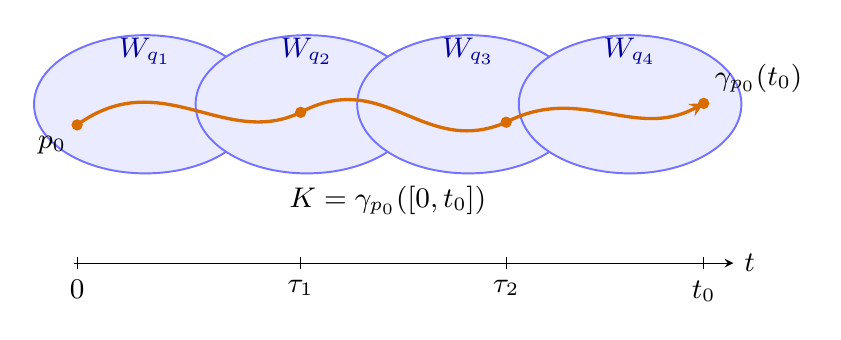
\begin{tikzpicture}[x=1cm,y=1cm,scale=1.14,transform shape,>=stealth,
    every node/.style={font=\small}]
  % Skończone pokrycie obrazu krzywej.
  \foreach \x/\i in {1.0/1,2.8/2,4.6/3,6.4/4}{
    \filldraw[fill=blue!8,draw=blue!55,line width=.7pt]
      (\x,1.75) ellipse (1.24 and .77);
    \node[blue!60!black] at (\x,2.34) {$W_{q_{\i}}$};
  }
  \draw[very thick,orange!85!black,->]
    (0.24,1.52) .. controls (1.18,2.20) and (1.88,1.25) .. (2.73,1.66)
    .. controls (3.67,2.16) and (4.10,1.15) .. (5.02,1.55)
    .. controls (5.85,1.98) and (6.45,1.34) .. (7.22,1.76);
  \fill[orange!85!black] (0.24,1.52) circle (1.8pt);
  \fill[orange!85!black] (2.73,1.66) circle (1.8pt);
  \fill[orange!85!black] (5.02,1.55) circle (1.8pt);
  \fill[orange!85!black] (7.22,1.76) circle (1.8pt);
  \node[below left] at (0.24,1.52) {$p_0$};
  \node[above right] at (7.22,1.76) {$\gamma_{p_0}(t_0)$};
  \node at (3.7,.68) {$K=\gamma_{p_0}([0,t_0])$};
  \draw[->] (.2,-.02)--(7.55,-.02) node[right] {$t$};
  \foreach \x/\lab in {.24/0,2.73/{\tau_1},5.02/{\tau_2},7.22/{t_0}}{
    \draw (\x,-.09)--(\x,.05);
    \node[below] at (\x,-.09) {$\lab$};
  }
\end{tikzpicture}

\caption{Skończone pokrycie zwartego obrazu $K$ otoczeniami,
na których obowiązuje wspólny dodatni czas lokalnego istnienia.
Podział czasu wybieramy dostatecznie drobny.}
\label{fig:przeplyw-pokrycie}
\end{figure}

Teraz dla każdego $j=0,\ldots,N-1$ oznaczmy
$z_j:=\gamma_{p_0}(\tau_j)$ i wybierzmy jeden ze zbiorów
$W_{q_i}$ zawierający $z_j$. Nazwijmy go $W_j$.
Lokalny przepływ odpowiadający temu otoczeniu oznaczmy przez
$L_j$. Ponieważ $\Delta_j<\varepsilon$, odwzorowanie
$\Psi_j\colon W_j\to M$, dane wzorem
$\Psi_j(z):=L_j(\Delta_j,z)$, jest gładkie.
Przesuwa ono punkt $z$ wzdłuż jego krzywej całkowej o czas
$\Delta_j$. Z jednoznaczności rozwiązań wynika w szczególności,
że $\Psi_j(z_j)=z_{j+1}$.

Musimy jednak uważać na dziedziny: obraz całego $W_j$ przez
$\Psi_j$ nie musi zawierać się w $W_{j+1}$. Nie możemy więc bez
dalszych przygotowań składać odwzorowań $\Psi_{j+1}$ i $\Psi_j$.
Rozwiązujemy ten problem, zmniejszając \emph{wyłącznie otoczenie
początkowego punktu $p_0$}, a nie zbiory $W_j$.

Rozpocznijmy od $U_0:=W_0$ i $F_0:=\id_{U_0}$.
Załóżmy indukcyjnie, że $U_j$ jest otwartym otoczeniem $p_0$,
a $F_j\colon U_j\to M$ jest gładkim odwzorowaniem opisującym
przesunięcie o czas $\tau_j$, przy czym $F_j(p_0)=z_j$.
Definiujemy
\[
U_{j+1}:=U_j\cap F_j^{-1}(W_j),\qquad
F_{j+1}:=\Psi_j\circ F_j\big|_{U_{j+1}}.
\]
Zbiór $U_{j+1}$ jest otwarty, ponieważ $F_j$ jest ciągłe
i $W_j$ jest otwarty. Zawiera $p_0$, gdyż
$F_j(p_0)=z_j\in W_j$. Co najważniejsze,
$F_j(U_{j+1})\subseteq W_j$, zatem następny lokalny przepływ
$\Psi_j$ rzeczywiście można zastosować do wszystkich punktów
z $U_{j+1}$. Odwzorowanie $F_{j+1}$ jest gładkie jako złożenie
odwzorowań gładkich i, na mocy jednoznaczności,
$F_{j+1}(p)=\gamma_p(\tau_{j+1})$ dla $p\in U_{j+1}$.

Dla lepszego zobrazowania pierwszych dwóch kroków oznaczmy
$p_j:=\gamma_{p_0}(\tau_j)$ i przyjmijmy
$\Psi_0(z)=\gamma_z(\tau_1-\tau_0)$,
$\Psi_1(z)=\gamma_z(\tau_2-\tau_1)$ na odpowiednich
otoczeniach $W_0$ i $W_1$. Wówczas
$U_1=U_0$ oraz $U_2=U_1\cap\Psi_0^{-1}(W_1)$. Jeśli dodatkowo wybierzemy
otoczenie $W_2$ punktu $p_2$, to
$U_3=U_2\cap(\Psi_1\circ\Psi_0)^{-1}(W_2)$
zapewnia możliwość wykonania kolejnego kroku po czasie $\tau_2$.
Rysunek~\ref{fig:przeplyw-skladanie-lokalne} pokazuje, skąd
biorą się kolejne ograniczenia otoczenia początkowego.

\begin{figure}[H]
\centering
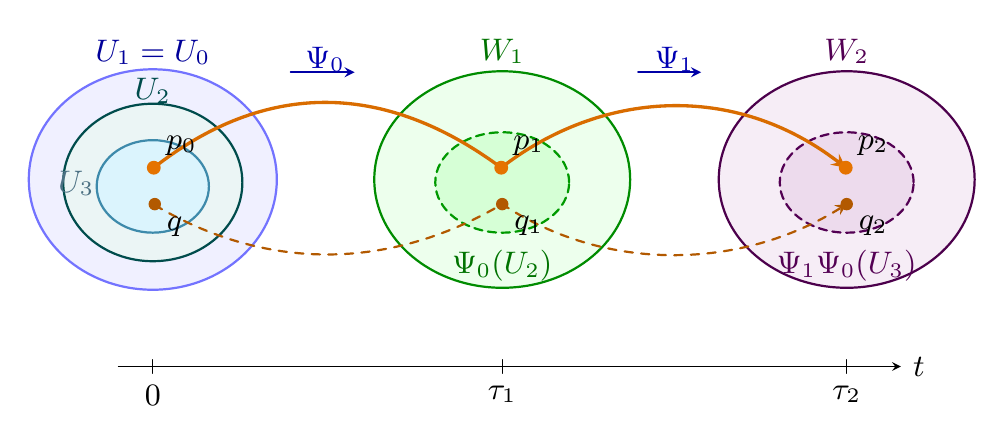
\begin{tikzpicture}[x=1cm,y=1cm,scale=1.25,transform shape,>=stealth,
    every node/.style={font=\small},line cap=round]
  % Otoczenia początkowe: U3 zawiera się w U2, a U2 w U1=U0.
  \filldraw[fill=blue!6,draw=blue!55,thick]
    (1.0,1.85) ellipse (1.26 and 1.12);
  \filldraw[fill=teal!8,draw=teal!60!black,thick]
    (1.0,1.82) ellipse (.91 and .80);
  \filldraw[fill=cyan!14,draw=cyan!65!black,thick]
    (1.0,1.78) ellipse (.57 and .47);
  \node[blue!60!black] at (1.0,3.14) {$U_1=U_0$};
  \node[teal!60!black] at (1.0,2.75) {$U_2$};
  \node[cyan!45!black,anchor=east] at (.53,1.81) {$U_3$};

  % Otoczenia w chwilach tau_1 i tau_2 oraz obrazy podzbiorów.
  \filldraw[fill=green!7,draw=green!55!black,thick]
    (4.55,1.85) ellipse (1.30 and 1.10);
  \filldraw[fill=green!16,draw=green!60!black,densely dashed,thick]
    (4.55,1.82) ellipse (.68 and .51);
  \node[green!45!black] at (4.55,3.15) {$W_1$};
  \node[green!45!black] at (4.55,.97) {$\Psi_0(U_2)$};

  \filldraw[fill=violet!7,draw=violet!60!black,thick]
    (8.05,1.85) ellipse (1.30 and 1.10);
  \filldraw[fill=violet!14,draw=violet!65!black,densely dashed,thick]
    (8.05,1.82) ellipse (.68 and .51);
  \node[violet!65!black] at (8.05,3.15) {$W_2$};
  \node[violet!65!black] at (8.05,.97) {$\Psi_1\Psi_0(U_3)$};

  % Krzywa bazowa i krzywa punktu pobliskiego q.
  \draw[orange!85!black,very thick,->]
    (1.01,1.97) .. controls (2.15,2.86) and (3.35,2.85) .. (4.54,1.97)
    .. controls (5.55,2.75) and (6.90,2.85) .. (8.04,1.97);
  \draw[orange!70!black,dashed,thick,->]
    (1.02,1.59) .. controls (2.20,.89) and (3.45,.95) .. (4.55,1.60)
    .. controls (5.60,.90) and (6.98,.93) .. (8.05,1.60);

  \foreach \x in {1.01,4.54,8.04}{
    \fill[orange!90!black] (\x,1.97) circle (2pt);
  }
  \foreach \x in {1.02,4.55,8.05}{
    \fill[orange!70!black] (\x,1.60) circle (1.8pt);
  }
  \node[above right] at (1.01,1.97) {$p_0$};
  \node[above right] at (4.54,1.97) {$p_1$};
  \node[above right] at (8.04,1.97) {$p_2$};
  \node[below right] at (1.02,1.59) {$q$};
  \node[below right] at (4.55,1.60) {$q_1$};
  \node[below right] at (8.05,1.60) {$q_2$};

  \node[blue!70!black] at (2.75,3.07) {$\Psi_0$};
  \node[blue!70!black] at (6.30,3.07) {$\Psi_1$};
  \draw[->,blue!65!black,semithick] (2.40,2.94)--(3.05,2.94);
  \draw[->,blue!65!black,semithick] (5.93,2.94)--(6.57,2.94);

  % Schematyczna oś czasu (nie jest osią współrzędnych M).
  \draw[->] (.65,-.05)--(8.60,-.05) node[right] {$t$};
  \foreach \x/\lab in {1.0/0,4.55/{\tau_1},8.05/{\tau_2}}{
    \draw (\x,-.12)--(\x,.02);
    \node[below] at (\x,-.12) {$\lab$};
  }
\end{tikzpicture}

\caption{Składanie dwóch lokalnych przesunięć w czasie.
Po lewej $p_0,q\in U_3\subseteq U_2\subseteq U_1=U_0$;
w środku $p_1=\Psi_0(p_0)$ i $q_1=\Psi_0(q)$
należą do $W_1$, a po prawej $p_2=\Psi_1(p_1)$
i $q_2=\Psi_1(q_1)$ należą do $W_2$.
Linia ciągła przedstawia krzywą przez $p_0$,
a przerywana krzywą przez $q$.}
\label{fig:przeplyw-skladanie-lokalne}
\end{figure}

W ten sposób, po skończenie wielu krokach, otrzymujemy otwarte
otoczenie $U_N$ punktu $p_0$, na którym
\[
\Phi_{t_0}(p)=F_N(p)
=\Psi_{N-1}\circ\cdots\circ\Psi_0(p),\qquad p\in U_N.
\]
Wszystkie złożenia są tu dobrze określone dzięki kolejnym
ograniczeniom dziedzin. Zatem $p\mapsto\Phi_{t_0}(p)$ jest gładkie
na $U_N$. Jest to jednak dopiero gładkość przy \emph{ustalonym}
czasie $t_0$.

Aby uzyskać gładkość względem obu zmiennych, wybierzmy otoczenie
$W_*$ punktu $z_N=\gamma_{p_0}(t_0)$ i liczbę $\delta>0$,
na których istnieje gładki lokalny przepływ
$L_*\colon(-\delta,\delta)\times W_*\to M$.
Ponieważ $F_N(p_0)=z_N\in W_*$ i $F_N$ jest ciągłe, zbiór
$V:=U_N\cap F_N^{-1}(W_*)$ jest otwartym otoczeniem $p_0$.
Dla $p\in V$ oraz $|u|<\delta$ możemy więc zdefiniować
$L_*(u,F_N(p))$. Jednoznaczność rozwiązań daje
\[
\Phi(t_0+u,p)=L_*(u,F_N(p)),
\qquad |u|<\delta,\quad p\in V.
\]
Prawa strona jest gładka łącznie względem $u$ i $p$,
gdyż jest złożeniem gładkich odwzorowań.
Ponadto wszystkie te rozwiązania istnieją dla wskazanych czasów,
co daje $(t_0-\delta,t_0+\delta)\times V\subseteq\mathcal D_X$.
Jeżeli $t_0<0$, powtarzamy argument z ujemnymi przyrostami czasu;
przy $t_0=0$ wystarcza lokalne twierdzenie o istnieniu.
Wobec dowolności $(t_0,p_0)$ dowiedliśmy jednocześnie, że
$\mathcal D_X$ jest otwarty i $\Phi$ jest gładkie.

\medskip
\noindent\emph{Przesunięcie czasu i prawo grupowe.}
Niech $s\in I_p$ i $q:=\Phi_s(p)$. Krzywa
$u\mapsto\gamma_p(s+u)$ jest określona na przedziale $I_p-s$,
spełnia równanie krzywej całkowej i w chwili $u=0$ przyjmuje
wartość $q$. Z jednoznaczności i maksymalności $\gamma_q$
wynika $I_p-s\subseteq I_q$ oraz
$\gamma_q(u)=\gamma_p(s+u)$ na $I_p-s$.
W szczególności $-s\in I_q$ i $\gamma_q(-s)=p$.

Możemy więc rozważyć krzywą
$v\mapsto\gamma_q(v-s)$, określoną na $s+I_q$.
W chwili $v=0$ przechodzi ona przez $p$. Jej maksymalność
w punkcie początkowym $p$ daje $s+I_q\subseteq I_p$.
Łącząc oba zawierania, otrzymujemy $I_q=I_p-s$ oraz
\[
\Phi_t(\Phi_s(p))=\gamma_q(t)=\gamma_p(s+t)=\Phi_{s+t}(p)
\qquad (t\in I_q).
\]
W szczególności $\Phi_0(p)=p$.
Równość przedziałów pokazuje też precyzyjnie, kiedy wolno
składać przepływy: dla danego $s\in I_p$ warunek
$t\in I_{\Phi_s(p)}$ jest równoważny $s+t\in I_p$.

\medskip
\noindent\emph{Dyfeomorfizmy i odwrotności.}
Dla każdego ustalonego $t$ zbiór $M_t$ jest otwarty:
jest przekrojem otwartego zbioru $\mathcal D_X$
przez odwzorowanie ciągłe $p\mapsto(t,p)$.
Jeśli $p\in M_t$ i $q=\Phi_t(p)$, to z udowodnionego wzoru
$I_q=I_p-t$ wynika $-t\in I_q$, czyli $q\in M_{-t}$.
Ponadto $\Phi_{-t}(q)=p$. Po zamianie $t$ na $-t$
otrzymujemy odwrotne zawieranie, zatem
$\Phi_t(M_t)=M_{-t}$ i
$\Phi_t^{-1}=\Phi_{-t}$. Oba odwzorowania są gładkie,
więc $\Phi_t\colon M_t\to M_{-t}$ jest dyfeomorfizmem.

\medskip
\noindent\emph{Pole jako generator przepływu.}
Z definicji krzywej całkowej mamy
$\left.\frac{\dd}{\dd t}\right|_{t=0}\Phi_t(p)
=\gamma_p'(0)=X_p$.
Aby otrzymać drugą równość w~\eqref{eq:przeplyw-generuje},
ustalmy $p\in M_t$. Dla $s$ dostatecznie bliskiego zeru
prawo składania daje
$\Phi_t(\Phi_s(p))=\Phi_s(\Phi_t(p))$.
Różniczkując tę tożsamość względem $s$ w zerze,
otrzymujemy z reguły łańcuchowej
$(\dd\Phi_t)_pX_p=X_{\Phi_t(p)}$.
Oznacza to, że różniczka przepływu przenosi wektor pola
w punkcie początkowym na wektor pola w jego obrazie.

\medskip
\noindent\emph{Przypadek pola zupełnego.}
Jeśli $X$ jest zupełne, to $I_p=\R$ dla każdego $p$,
a więc $\mathcal D_X=\R\times M$ oraz $M_t=M$.
Z udowodnionych własności wynika wówczas
$\Phi_{t+s}=\Phi_t\circ\Phi_s$,
$\Phi_0=\id_M$ i $\Phi_t^{-1}=\Phi_{-t}$.
W szczególności $t\mapsto\Phi_t$ jest homomorfizmem
$(\R,+)\to\operatorname{Diff}(M)$, natomiast
$(t,p)\mapsto\Phi_t(p)$ jest gładkim działaniem grupy
$(\R,+)$ na $M$. Dla pola niezupełnego te same tożsamości
obowiązują tylko tam, gdzie wszystkie ich strony są określone.
\end{proof}

\begin{stwierdzenie}[Grupa przepływu wyznacza swoje pole]
Jeśli gładkie odwzorowanie $H\colon\R\times M\to M$ spełnia
$H_0=\id_M$ oraz $H_{t+s}=H_t\circ H_s$ dla wszystkich
$t,s\in\R$, to wzór
$X_p:=\left.\frac{\dd}{\dd t}\right|_{t=0}H_t(p)$
określa gładkie zupełne pole wektorowe $X$, którego
przepływem jest $H$, tzn. $H_t=\Phi_t^X$ dla każdego $t\in\R$.
\end{stwierdzenie}

\begin{proof}
Z prawa grupowego wynika
$H_t\circ H_{-t}=H_{-t}\circ H_t=\id_M$, więc każde $H_t$
jest dyfeomorfizmem o odwrotności $H_{-t}$.
Gładkość $H$ pociąga za sobą gładkość pola $X$,
ponieważ w lokalnych współrzędnych jego składowe są pochodnymi
cząstkowymi składowych $H$ względem czasu w zerze.

Dla ustalonego $p$ mamy $H_{t+h}(p)=H_h(H_t(p))$.
Różniczkując obie strony względem $h$ w chwili $h=0$,
dostajemy
\[
\frac{\dd}{\dd t}H_t(p)=X_{H_t(p)},\qquad H_0(p)=p.
\]
Zatem $t\mapsto H_t(p)$ jest krzywą całkową pola $X$,
określoną na całej prostej. Z jednoznaczności maksymalnej krzywej
wynika $H_t(p)=\Phi_t^X(p)$ dla wszystkich $t\in\R$.
Pole $X$ jest więc zupełne.
\end{proof}

Rysunek~\ref{fig:przeplyw-przekroj} pokazuje działanie $\Phi_t$
na przekroju poprzecznym do krzywych całkowych.
\begin{figure}[H]
\centering
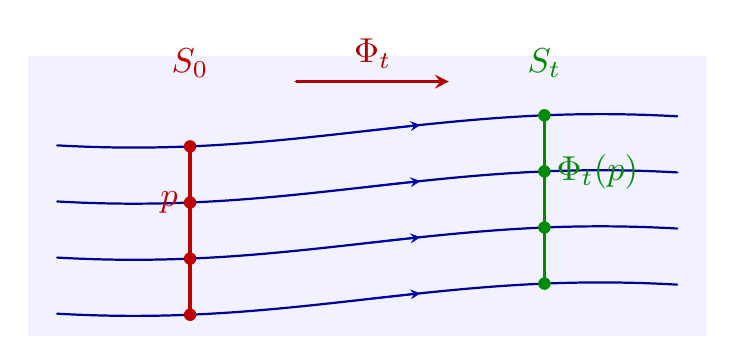
\begin{tikzpicture}[x=1cm,y=1cm,scale=1.25,transform shape,>=stealth,line cap=round]
  \fill[blue!5] (-3.45,-1.42) rectangle (3.45,1.42);
  \foreach \c in {-1.05,-.48,.09,.66}{
    \draw[blue!58!black,thick]
       plot[domain=-3.15:3.15,samples=55]
       ({\x},{\c+.17*sin(38*\x)});
    \draw[->,blue!70!black,semithick]
       (0,{\c}) -- (.54,{\c+.17*sin(38*.54)});
  }
  \draw[red!75!black,very thick]
      (-1.8,{-1.05+.17*sin(38*(-1.8))}) --
      (-1.8,{.66+.17*sin(38*(-1.8))});
  \draw[green!55!black,very thick]
      (1.8,{-1.05+.17*sin(38*1.8)}) --
      (1.8,{.66+.17*sin(38*1.8)});
  \foreach \c in {-1.05,-.48,.09,.66}{
    \fill[red!75!black] (-1.8,{\c+.17*sin(38*(-1.8))}) circle (1.8pt);
    \fill[green!55!black] (1.8,{\c+.17*sin(38*1.8)}) circle (1.8pt);
  }
  \node[red!75!black,above] at (-1.8,1.08) {$S_0$};
  \node[green!55!black,above] at (1.8,1.08) {$S_t$};
  \node[red!75!black,left] at (-1.8,{.09+.17*sin(38*(-1.8))}) {$p$};
  \node[green!55!black,right] at (1.8,{.09+.17*sin(38*1.8)}) {$\Phi_t(p)$};
  \draw[->,red!70!black,very thick]
      (-.72,1.16)--(.83,1.16) node[midway,above] {$\Phi_t$};
\end{tikzpicture}

\caption{Przepływ przesuwa przekrój poprzeczny $S_0$
na przekrój $S_t$, prowadząc każdy punkt wzdłuż jego krzywej
całkowej. Pokazane krzywe są trajektoriami pola
$X=(1,A\kappa\cos(\kappa x))$, gdzie $A=0.17$,
$\kappa=38\pi/180$. Jego przepływ ma postać
$\Phi_s(x,y)=(x+s,y+A[\sin(\kappa(x+s))-\sin(\kappa x)])$;
na rysunku $t=3.6$.}
\label{fig:przeplyw-przekroj}
\end{figure}

\begin{przyklad}[Trzy zupełne przepływy]
Na $\R^n$ pole stałe $X=v$ ma $\Phi_t(x)=x+tv$:
pochodna po $t$ jest równa $v$, niezależnie od położenia.
Pole Eulera $E=\sum_i x^i\partial_i$ ma $\Phi_t(x)=e^t x$,
bo $\frac{\dd}{\dd t}(e^t x)=e^t x=E_{e^t x}$.
Pole obrotowe z~\eqref{eq:obrot} ma
$\Phi_t(a,b)=(a\cos t-b\sin t,a\sin t+b\cos t)$.
Wszystkie trzy wzory są określone dla całego $t\in\R$ i
spełniają $\Phi_0=\id$ oraz $\Phi_{t+s}=\Phi_t\circ\Phi_s$.
\end{przyklad}

\begin{przyklad}[Ucieczka w skończonym czasie]\label{prz:niezupelne}
Dla $X=x^2\partial_x$ na $\R$ krzywa przez $x_0$ spełnia
\[
 \Phi_t(x_0)=\frac{x_0}{1-tx_0}
 \qquad\text{w maksymalnym przedziale zawierającym }0.
\]
Rzeczywiście, pochodna ilorazu wynosi
$x_0^2/(1-tx_0)^2=\Phi_t(x_0)^2$, a w chwili zero
otrzymujemy $x_0$. Dla $x_0=0$ ten sam wzór daje krzywą stałą.
Jeśli $x_0>0$, jej dziedzina to $(-\infty,1/x_0)$; jeśli $x_0<0$,
to $(1/x_0,\infty)$; dla $x_0=0$ jest nią $\R$.
Zatem dziedzina całego przepływu ma prosty opis
\[
\mathcal D_X=\{(t,x_0)\in\R^2:1-tx_0>0\}.
\]
Jest otwarta, ale nie jest iloczynem przedziału czasu i
całej prostej: czas, do którego dociera krzywa, zależy od $x_0$.
Dla ustalonego $t$ dziedziną $\Phi_t$ jest dokładnie
$M_t=\{x_0\in\R:1-tx_0>0\}$; dla $t=0$ jest to cała $\R$.
Algebraiczny wzór na $\Phi_t(x_0)$ ma też wartość przy
$1-tx_0<0$, lecz oddziela ją od chwili początkowej biegun
$t=1/x_0$; nie należy do tej samej krzywej całkowej.
Pole jest gładkie na całej prostej,
ale nie jest zupełne: nieograniczony wzrost rozwiązania powoduje
ucieczkę do nieskończoności w skończonym czasie.
\end{przyklad}

\begin{twierdzenie}[Kryterium przedłużenia i dwa warunki zupełności]
\label{thm:zupelnosc}
Jeśli maksymalna krzywa całkowa ma skończony prawy koniec $b$, to
opuszcza w pobliżu $b$ każdy zwarty podzbiór $M$.
W konsekwencji każde pole na rozmaitości zwartej jest zupełne.
Każde pole o zwartym nośniku na dowolnej rozmaitości także jest zupełne.
\end{twierdzenie}
\begin{proof}
\emph{Kryterium przedłużenia.}
Niech $I_p=(a,b)$ i $b<\infty$. Załóżmy przeciwnie,
że istnieją zbiór zwarty $K\subset M$ i ciąg
$t_j\nearrow b$ taki, że $\gamma_p(t_j)\in K$.
Po wybraniu podciągu mamy $\gamma_p(t_j)\to q\in K$.
Lokalne twierdzenie o istnieniu w $q$ daje otoczenie
$W\ni q$ i $\varepsilon>0$ takie, że z każdego punktu
$W$ można prowadzić rozwiązanie przez wszystkie czasy
$u\in(-\varepsilon,\varepsilon)$.
Dla dużego $j$ zachodzi $\gamma_p(t_j)\in W$
oraz $b-t_j<\varepsilon/2$.
Krzywa
\[
 u\longmapsto\Phi_u(\gamma_p(t_j)),\qquad
 -\varepsilon<u<\varepsilon,
\]
pokrywa się z $u\mapsto\gamma_p(t_j+u)$ w ich wspólnej
dziedzinie, bo obie zaczynają w $\gamma_p(t_j)$.
Możemy więc skleić je w krzywą określoną także dla
$t> b$, sprzecznie z maksymalnością $I_p$.
Przy skończonym lewym końcu stosujemy ten sam argument
do pola $-X$ i czasu odwróconego.

\emph{Zupełność na zbiorach zwartych.}
Jeśli $M$ jest zwarta, każda trajektoria przez cały czas
leży w jednym zwartym zbiorze $M$. Kryterium wyklucza
oba skończone końce $I_p$, zatem $I_p=\R$.
Teraz niech $K=\supp X$ będzie zwarty.
Jeśli $p\notin K$, to $X_p=0$, więc krzywa
stała w $p$ jest, z jednoznaczności, całą krzywą
maksymalną. Jeśli $p\in K$, krzywa nie może wejść
do $M\setminus K$: od chwili wejścia byłaby stała,
a jednoznaczność, zastosowana także wstecz w czasie,
zmusiłaby ją do bycia stałą już w chwili zero.
W obu przypadkach obraz $\gamma_p$ leży w zwartym
zbiorze $K\cup\{p\}$; kryterium znów daje $I_p=\R$.
\end{proof}

\begin{uwaga}[Nie mylić zupełności z brakiem zer]
Zupełne pole może mieć zera (obrót na płaszczyźnie), a pole bez zer
może być niezupełne, np.\ $X=(1+x^2)\partial_x$ na $\R$.
Dla rozmaitości z brzegiem pole musi dodatkowo być styczne do brzegu,
aby dać dwustronny przepływ zachowujący tę rozmaitość.
Istotnie, dyfeomorfizmy zachowują brzeg, więc różniczkowanie
krzywej $t\mapsto\Phi_t(p)$ dla $p\in\partial M$ daje
$X_p\in T_p\partial M$. Odwrotnie, dla pola stycznego do brzegu
rozwiązujemy równanie również na $\partial M$; jednoznaczność
w lokalnym przedłużeniu pola zapewnia, że jego krzywe przez
brzeg pozostają na brzegu. Krzywe z wnętrza nie mogą go
przekroczyć, bo przy pierwszym spotkaniu jednoznaczność wstecz
wymuszałaby wcześniejszy pobyt na brzegu.
Pole skierowane do wnętrza na brzegu daje zwykle przepływ tylko
dla małych dodatnich czasów, co wykorzystamy do budowania kołnierza.
Na przykład na $M=[0,\infty)$ pole $X=\partial_r$ jest gładkim
przekrojem pełnej wiązki stycznej, także w $0$.
Krzywa całkowa zaczynająca się w $0$ musiałaby mieć postać
$r(t)=t$, więc dla $t<0$ opuszczałaby $M$.
Nie ma tu sprzeczności ze Stwierdzeniem~\ref{prop:styczna-brzeg-1}:
$T_0M\cong\R$, ale $T_0\partial M=\{0\}$ i $X_0\notin T_0\partial M$.
Styczność do brzegu zapewnia lokalny przepływ dwustronny;
jego istnienie dla wszystkich czasów wymaga ponadto zupełności.
\end{uwaga}

\section{Geometria przepływu: prostowanie, niezmienniki, komutowanie}
\label{sec:prostowanie}

\begin{definicja}[Orbita i nasycenie przez przepływ]
\index{orbita i nasycenie przez przeplyw@Orbita i nasycenie przez przepływ}
\emph{Orbitą} punktu $p$ pod przepływem pola $X$ jest
$\mathcal O_X(p)=\{\Phi_t(p):t\in I_p\}$.
Dla $A\subseteq M$ jego \emph{nasycenie przez przepływ}
to suma orbit punktów z $A$:
\[
 \operatorname{Sat}_X(A)=\bigcup_{p\in A}\mathcal O_X(p).
\]
Zbiór $A$ jest \emph{nasycony przez $X$}, gdy
$\operatorname{Sat}_X(A)=A$, czyli gdy
$p\in A$ i $t\in I_p$ pociągają za sobą
$\Phi_t(p)\in A$.
\end{definicja}

To jest nasycenie względem relacji ,,leżeć na tej samej
orbicie'' w sensie Definicji~\ref{def:nasycenie}.
Istotnie, gdy $q=\Phi_s(p)$, to
$I_q=I_p-s$ i $\mathcal O_X(q)=\mathcal O_X(p)$
na mocy Twierdzenia~\ref{thm:przeplyw}; orbity rozcinają
więc $M$ na rozłączne klasy. Na przykład dla
$X=\partial_x$ na $\R^2$ nasyceniem
$\{0\}\times(0,1)$ jest cały pas $\R\times(0,1)$.

\begin{twierdzenie}[Twierdzenie o prostowaniu pola]\label{thm:flowbox}
Jeśli $X_p\ne0$, to istnieją współrzędne $(t,z^2,\ldots,z^n)$
w otoczeniu $p$, w których $X=\partial_t$. W tych współrzędnych
lokalny przepływ ma postać
\[
 (t,z^2,\ldots,z^n)\longmapsto(t+s,z^2,\ldots,z^n).
\]
\end{twierdzenie}
\begin{proof}
Wybieramy małą $(n-1)$-wymiarową podrozmaitość $S$
przechodzącą przez $p$ i poprzeczną do $X_p$, oraz parametryzację
$\sigma\colon V\subset\R^{n-1}\to S$ z $\sigma(0)=p$.
Można ją zbudować bez dodatkowego twierdzenia: wybieramy mapę
z $p=0$ i po liniowej zmianie współrzędnych z pierwszą składową
$X_p$ niezerową; bierzemy $S=\{x^1=0\}$ w tej mapie.
Odwzorowanie $F(t,z)=\Phi_t(\sigma(z))$ ma w $(0,0)$
różniczkę, której pierwszą kolumną jest $X_p$, a pozostałe kolumny
rozpinają $T_pS$. Jest więc izomorfizmem. Z twierdzenia o funkcji
odwrotnej $F$ jest lokalnym dyfeomorfizmem. Zmniejszamy jego
dziedzinę do produktu $(-\varepsilon,\varepsilon)\times V_0$.
Ponieważ $\partial_tF(t,z)=X_{F(t,z)}$, we współrzędnych $F^{-1}$
pole ma postać $\partial_t$. Prawo grupowe daje
$\Phi_s(F(t,z))=F(t+s,z)$, dopóki $t$ i $t+s$ leżą
w tym przedziale. To wyjaśnia lokalny zakres wzoru z tezy.
\end{proof}

Współrzędna $t$ mierzy czas ruchu od poprzecznego przekroju,
a $z=(z^2,\ldots,z^n)$ wskazuje punkt tego przekroju.
Gładką funkcję $h$ spełniającą $X(h)=0$ na otwartym zbiorze
\index{pierwsza calka@Pierwsza całka}
nazywamy tam \emph{całką pierwszą} pola: jej wartość nie zmienia się
wzdłuż żadnej trajektorii w tym zbiorze.
W prostującym otoczeniu trajektorie mają stałe $z$;
każda składowa $z^i$ jest więc lokalną całką pierwszą.

\begin{przyklad}[Jawne współrzędne prostujące]
Na $\R^2$ rozważmy pole
$X=\partial_x+y\partial_y$.
Jego krzywe całkowe spełniają $x'=1$, $y'=y$, więc
\[
\Phi_t(x_0,y_0)=(x_0+t,e^t y_0),
\qquad t\in\R.
\]
Jako przekrój poprzeczny wybieramy $S=\{x=0\}$ z
parametryzacją $\sigma(z)=(0,z)$.
Konstrukcja z dowodu Twierdzenia~\ref{thm:flowbox} daje
\[
F(t,z)=\Phi_t(\sigma(z))=(t,e^t z),
\qquad F^{-1}(x,y)=(x,e^{-x}y).
\]
W tym przykładzie $F$ jest dyfeomorfizmem całej $\R^2$,
więc prostowanie działa globalnie. Nowa współrzędna
$z=e^{-x}y$ nie zmienia się wzdłuż ruchu; bezpośrednio
\[
X(z)=\partial_x(e^{-x}y)+y\partial_y(e^{-x}y)
=-e^{-x}y+ye^{-x}=0.
\]
Orbity mają równania $y=Ce^x$, gdzie $C=z$ jest wartością
punktu przecięcia z $S$. Dla przedziału $(a,b)\subset\R$
nasycenie fragmentu przekroju jest zatem
\[
\operatorname{Sat}_X(\{0\}\times(a,b))
=\{(x,y)\in\R^2:a<e^{-x}y<b\}.
\]
Na Rysunku~\ref{fig:prostowanie-pola-przyklad} widać,
dlaczego współrzędna $z$ etykietuje trajektorie, a $t$
opisuje ruch po każdej z nich.
\end{przyklad}

\begin{figure}[!htbp]
\centering
\begin{tikzpicture}[>=Stealth,x=1.35cm,y=.85cm,line cap=round]
  \draw[->,black!55] (-1.6,0)--(1.7,0) node[right,font=\small] {$x$};
  \draw[->,black!55] (0,-2.55)--(0,2.65) node[above,font=\small] {$y$};
  \draw[manifoldgold!75!black,very thick] (0,-2.35)--(0,2.42);
  \foreach \c in {-.55,0,.55}{
    \draw[manifoldblue!75!black,thick]
      plot[domain=-1.45:1.45,samples=60] (\x,{\c*exp(\x)});
  }
  \draw[->,manifoldred,very thick]
    plot[domain=0:.82,samples=35] (\x,{.55*exp(\x)});
  \fill[manifoldred] (0,.55) circle (2.3pt)
    node[above left,font=\small] {$p=\sigma(z)$};
  \fill[manifoldred] (.82,{.55*exp(.82)}) circle (2.3pt)
    node[above right,font=\small] {$\Phi_t(p)$};
  \node[manifoldgold!75!black,font=\small,anchor=west]
    at (.08,2.32) {$S=\{x=0\}$};
  \node[manifoldblue!75!black,font=\small] at (1.48,-1.95)
    {$y=Ce^x$};
\end{tikzpicture}
\caption{Pole $X=\partial_x+y\partial_y$: niebieskie krzywe są
orbitami $y=Ce^x$. Każda przecina złoty przekrój $S$ w jednym
punkcie $(0,C)$. Czerwony łuk pokazuje ruch od $p$ do $\Phi_t(p)$;
współrzędna $z=C$ pozostaje na nim stała.}
\label{fig:prostowanie-pola-przyklad}
\end{figure}

\begin{uwaga}
Pola nie można wyprostować w zerze $X_p=0$: dyfeomorfizm przenosi
wektor zerowy na wektor zerowy, natomiast $\partial_t$ nigdzie
nie znika. W zerze lokalne trajektorie i zachowanie przepływu
bada się innymi metodami niż prostowanie pola.
\end{uwaga}

\begin{stwierdzenie}[Lokalne twierdzenie Frobeniusa]
\label{prop:frobenius-lokalny}
Gładki rozkład inwolutywny $\mathcal D$ stałego rzędu $k$
ma lokalnie współrzędne, w których jest rozpięty przez pierwsze
$k$ pól współrzędnych.
\end{stwierdzenie}
\begin{proof}
Przeprowadzimy indukcję po $k$, jednocześnie dla wszystkich
wymiarów rozmaitości. Dla $k=0$ teza jest natychmiastowa.
Dla $k\ge1$ wybieramy lokalną bazę $X_1,\ldots,X_k$ rozkładu
i prostujemy niezerowe $X_1$. Mamy więc współrzędne $(t,z)$
w produkcie wokół $(0,0)$, z $X_1=\partial_t$.
Od każdego $X_j$, $j\ge2$, odejmujemy jego składową w kierunku
$\partial_t$. Otrzymane pola $Y_2,\ldots,Y_k$ nie mają tej
składowej, a wraz z $\partial_t$ nadal stanowią bazę $\mathcal D$.
Jeśli $k=1$, dowód jest już zakończony.

Niech $B(t,z)$ będzie macierzą o $k-1$ kolumnach złożonych
ze składowych $Y_2,\ldots,Y_k$ w kierunkach $z$.
Inwolutywność daje $[\partial_t,Y_j]\in\mathcal D$;
ponieważ ten nawias nie ma składowej czasowej, jest kombinacją
samych $Y_2,\ldots,Y_k$. Zatem
\[
 \partial_tB(t,z)=B(t,z)A(t,z)
\]
dla pewnej gładkiej macierzy kwadratowej $A$.
Gładkość współczynników wynika z rozwiązania układu za pomocą
niezerowego minora macierzy $B$, po zmniejszeniu otoczenia.
Rozwiązujemy macierzowe równanie
\[
 \partial_tQ(t,z)=-A(t,z)Q(t,z),\qquad Q(0,z)=I.
\]
Istnienie i gładka zależność od $z$ wynikają z
Twierdzenia~\ref{thm:ode}: dołączamy zmienne z równaniami
$t'=1$, $z'=0$. Po zmniejszeniu produktu $Q$ jest odwracalna,
bo $Q(0,0)=I$. Reguła iloczynu daje
\[
 \partial_t(BQ)=BAQ-BAQ=0,\qquad B(t,z)Q(t,z)=B(0,z).
\]
Kolumny $BQ$ wyznaczają więc nową bazę pól pionowych
niezależnych od $t$, rozpinającą te same kierunki co kolumny $B$.
Na przekroju $t=0$ tworzą rozkład rzędu $k-1$.
Jest on inwolutywny: nawiasy tych pól nie mają składowej
czasowej, należą do $\mathcal D$ i nie zależą od $t$;
reguła Leibniza dla nawiasu rozszerza to na dowolne sekcje.
Z założenia indukcyjnego istnieje zmiana współrzędnych $z$
prostująca ten rozkład. Stosujemy ją niezależnie od $t$.
Ponieważ baza pionowa nie zależy od czasu, w całym produkcie
$\mathcal D$ jest rozpięty przez $\partial_t$ i pierwsze
$k-1$ nowych pól współrzędnych na przekroju. To kończy indukcję.
\end{proof}

\begin{stwierdzenie}[Funkcje i pola niezmiennicze]\label{prop:inwarianty}
Dla zupełnego $X$ gładka funkcja $f\in C^\infty(M)$ jest stała na każdej jego trajektorii
wtedy i tylko wtedy, gdy $X(f)=0$. Przepływ zawsze zachowuje
pole, które go generuje: $(\Phi_t)_*X=X$.
Dla innego pola $Y$ następujące warunki są równoważne:
\begin{enumerate}[label=(\roman*)]
\item $[X,Y]=0$;
\item $(\Phi_t)_*Y=Y$ dla wszystkich $t$;
\item dla każdego $p\in M$ i $t\in\R$ zachodzi
$I^Y_{\Phi_t^X(p)}=I^Y_p$ oraz
$\Phi_t^X(\Phi_s^Y(p))=\Phi_s^Y(\Phi_t^X(p))$
dla każdego $s\in I^Y_p$.
\end{enumerate}
Jeśli także $Y$ jest zupełne, ostatni punkt oznacza
$\Phi_t^X\circ\Phi_s^Y=\Phi_s^Y\circ\Phi_t^X$ dla wszystkich $s,t\in\R$.
\end{stwierdzenie}
\begin{proof}
Reguła łańcucha daje
$\frac{\dd}{\dd t}f(\Phi_t(p))=X(f)(\Phi_t(p))$.
Jeśli $X(f)=0$, funkcja czasu jest stała na $\R$;
odwrotnie, stałość każdej trajektorii daje pochodną zerową w $t=0$.
Druga równość wynika z~\eqref{eq:przeplyw-generuje}.

Wykażmy (i)$\Leftrightarrow$(ii) bez porównywania wektorów
z różnych przestrzeni stycznych. Ustalmy $p$ i oznaczmy
$\gamma(t)=\Phi_t^X(p)$. Na krótkim fragmencie krzywej
w jednej mapie traktujemy pola jako funkcje o wartościach w $\R^n$.
Oznaczmy tam
\[
V(t)=(\dd\Phi_t^X)_pY_p,
\qquad W(t)=Y_{\gamma(t)}.
\]
Równanie wariacyjne z dowodu Twierdzenia~\ref{thm:ode}
daje $V'(t)=\D X(\gamma(t))V(t)$.
Reguła łańcucha daje natomiast
$W'(t)=\D Y(\gamma(t))X_{\gamma(t)}$.
W tych samych współrzędnych wzór~\eqref{eq:nawias-wspolrzedne}
przyjmuje postać $[X,Y]=\D Y\,X-\D X\,Y$.
Jeśli (i) zachodzi, to $W'=\D X(\gamma)W$.
Ponieważ $V(0)=W(0)=Y_p$, jednoznaczność liniowego ODE
daje $V=W$ na pierwszym fragmencie. Na jego końcu są one
tym samym wektorem w $T_{\gamma(t)}M$, więc stanowią wspólną
wartość początkową po przejściu do następnej mapy.
Skończone pokrycie każdego zwartego odcinka czasu pozwala
powtórzyć argument aż do dowolnego $t$. Dostajemy
$(\dd\Phi_t^X)_pY_p=Y_{\Phi_t^X(p)}$ dla każdego $t$,
czyli (ii). Odwrotnie, przy (ii) mamy $V=W$;
porównanie ich pochodnych w $t=0$ daje
$\D X(p)Y_p=\D Y(p)X_p$, a więc $[X,Y]_p=0$.

Niech $\Psi_s$ oznacza maksymalny przepływ $Y$. Przy (ii)
dla każdego ustalonego $t$ krzywa $s\mapsto\Phi_t(\Psi_s(p))$
ma pochodną $\dd\Phi_t(Y)=Y$ i zaczyna w $\Phi_t(p)$.
Jednoznaczność i maksymalność dają
$I_p^Y\subseteq I_{\Phi_t(p)}^Y$ oraz
$\Phi_t(\Psi_s(p))=\Psi_s(\Phi_t(p))$ dla $s\in I_p^Y$.
Ponieważ $\Phi_t$ jest globalnym dyfeomorfizmem, zastosowanie
tego samego argumentu do $\Phi_{-t}$ daje odwrotne zawieranie
przedziałów. Otrzymaliśmy więc (iii) wraz ze zgodnością dziedzin.
Różniczkując (iii) po $s$ w zerze, odzyskujemy
$\dd\Phi_t(Y_p)=Y_{\Phi_t(p)}$, czyli (ii).
\end{proof}

Przy niezupełnym $X$ równości o zachowaniu pola i komutowaniu
pozostają lokalne: stosujemy je na wspólnej dziedzinie, na której
wszystkie występujące przepływy i ich złożenia są określone.

\begin{przyklad}[Dwa komutujące przepływy]
Wróćmy do $X=\partial_x+y\partial_y$ z przykładu prostowania
i weźmy $Y=y\partial_y$ na $\R^2$.
Współrzędnościowy wzór na nawias daje
\[
[X,Y]=[\partial_x+y\partial_y,y\partial_y]
=\bigl(X(y)-Y(y)\bigr)\partial_y=0.
\]
Przepływ $Y$ ma postać $\Psi_s(x,y)=(x,e^s y)$ i jest zupełny.
Oba złożenia można obliczyć bezpośrednio:
\[
\Phi_t(\Psi_s(x,y))=(x+t,e^{t+s}y)
=\Psi_s(\Phi_t(x,y)).
\]
W prostujących współrzędnych $(t,z)=(x,e^{-x}y)$
pole $X$ przesuwa tylko $t$, a $Y=z\partial_z$ zmienia
tylko $z$; stąd ich ruchy mają niezależne kierunki.
\end{przyklad}

\begin{przyklad}[Pierwsza całka]
Dla pola obrotowego $R=-y\partial_x+x\partial_y$
funkcja $f(x,y)=x^2+y^2$ spełnia $R(f)=0$.
Jej dodatnie poziomice są okręgami, po których biegnie przepływ;
poziomica zerowa to nieruchomy punkt $(0,0)$, a ujemne są puste.
Jest to globalna pierwsza całka pola obrotowego.
W ogólności poziomica pierwszej całki może zawierać kilka orbit:
dla $X=\partial_x$ na $\R^2$ funkcja $h(x,y)=y^2$ spełnia
$X(h)=0$, lecz poziomica $h^{-1}(1)$ składa się z dwóch
oddzielnych orbit $y=1$ i $y=-1$.
\end{przyklad}

\section{Pochodna Liego: porównywanie danych w różnych punktach}
\label{sec:liego}

Nie można po prostu odjąć wektorów $Y_{\Phi_t(p)}$ i $Y_p$:
należą do różnych przestrzeni stycznych. Przepływ $X$ dostarcza
\emph{kanonicznego w tej sytuacji} sposobu ich porównania:
różniczka odwrotnego przepływu przenosi pierwszy z nich do $T_pM$.
Otrzymujemy odpowiedź na pytanie, jak obiekt zmienia się
wraz z ruchem generowanym przez $X$.

\begin{definicja}\label{def:pochodna-liego}
\index{pochodna Liego@Pochodna Liego}
Dla funkcji $f$ i pola $Y$ określamy
\begin{align}
 (\Lie_Xf)(p)
 &=\left.\frac{\dd}{\dd t}\right|_{0}f(\Phi_t(p))=X(f)(p),
 \label{eq:lie-f}\\
 (\Lie_XY)_p
 &=\left.\frac{\dd}{\dd t}\right|_{0}
 (\dd\Phi_{-t})_{\Phi_t(p)}Y_{\Phi_t(p)}.
 \label{eq:lie-y}
\end{align}
Definicja jest lokalna: przepływ jest potrzebny tylko dla małego $t$.
Wzór~\eqref{eq:lie-y} zapisujemy krótko jako
$\Lie_XY=\left.\frac{\dd}{\dd t}\right|_0\Phi_t^*Y$.
\end{definicja}


\begin{figure}[!htbp]
\centering
\begin{tikzpicture}[>=Stealth,scale=1.06,line cap=round,line join=round]
% Jedno spójne otoczenie na M; p i q są punktami czerwonej trajektorii.
\filldraw[fill=manifoldblue!8,draw=manifoldblue!70!black,thick]
 (-5.14,-.67) .. controls (-5.15,.52) and (-4.33,1.28) .. (-3.3,1.26)
 .. controls (-1.92,1.22) and (-.88,1.39) .. (.37,1.16)
 .. controls (1.84,1.25) and (4.49,1.43) .. (5.03,.41)
 .. controls (5.52,-.42) and (4.83,-1.3) .. (3.44,-1.43)
 .. controls (1.94,-1.58) and (.42,-1.21) .. (-1.01,-1.44)
 .. controls (-2.84,-1.68) and (-4.84,-1.38) .. cycle;
\node[font=\small,manifoldblue!75!black] at (-4.8,1.51) {$M$};
\coordinate (P) at (-3.65,-.52);
\coordinate (Q) at (3.2,-.48);
% Ciągła krzywa całkowa; wyraźne punkty p, q i kierunek czasu.
\draw[manifoldred!40,thick] (-4.73,-.8)
 .. controls (-4.38,-.71) and (-3.96,-.57) .. (P);
\draw[manifoldred,very thick,postaction={decorate},
 decoration={markings,mark=at position .55 with {\arrow{Stealth}}}]
 (P) .. controls (-2.43,-.1) and (-1.21,-.69) .. (-.1,-.67)
 .. controls (1.13,-.63) and (2.08,-.12) .. (Q);
\draw[manifoldred!40,thick] (Q)
 .. controls (3.81,-.55) and (4.19,-.67) .. (4.67,-.66);
\node[font=\small,manifoldred!85!black] at (.14,-1.08)
 {$\gamma(s)=\Phi_s^X(p)$};
\fill[manifoldred] (P) circle (2.6pt)
 node[below left,font=\small] {$p=\gamma(0)$};
\fill[manifoldred] (Q) circle (2.6pt)
 node[below right,font=\small] {$q=\gamma(t)$};
% Wektory porównywane po sprowadzeniu do T_p M.
\draw[->,manifoldblue,very thick] (P)--(-4.06,.67);
\draw[->,manifoldgold!85!black,very thick] (P)--(-2.78,.78);
\node[font=\small,manifoldblue] at (-4.52,.86) {$Y_p$};
\node[font=\small,manifoldgold!80!black] at (-2.05,.65)
 {$\widetilde Y_t(p)$};
\draw[->,manifoldred,thick] (-4.06,.67)--(-2.78,.78);
\node[font=\small,manifoldred!85!black] at (-3.46,1.01) {$\Delta_t(p)$};
% Wektor Y_q oraz schemat cofnięcia jego wartości, odrębny od trajektorii.
\draw[->,manifoldblue,very thick] (Q)--(3.48,.83);
\node[font=\small,manifoldblue] at (3.98,.89) {$Y_q$};
\draw[->,manifoldgold!85!black,thick,densely dashed]
 (3.48,.83) .. controls (1.93,1.95) and (-.88,2.05) .. (-2.78,.78);
\node[font=\small,manifoldgold!80!black] at (.41,1.92)
 {$(\dd\Phi_{-t}^X)_q$};
\end{tikzpicture}
\caption{Punkty $p=\gamma(0)$ i $q=\gamma(t)=\Phi_t^X(p)$ leżą
na tej samej krzywej całkowej na $M$; czerwona strzałka pokazuje
ruch w czasie od $p$ do $q$. Wektor $Y_q$ cofamy różniczką
przepływu do $T_pM$, otrzymując $\widetilde Y_t(p)$.
Tam porównujemy go z $Y_p$; $\Delta_t(p)$ jest ich różnicą.
Przerywana strzałka przedstawia transport wektora, nie ruch punktu.}
\label{fig:pochodna-liego}
\end{figure}

Dokładnie, oznaczając $q=\Phi_t^X(p)$, mamy
\[
 \widetilde Y_t(p):=(\dd\Phi_{-t}^X)_qY_q\in T_pM,\qquad
 (\Lie_XY)_p=\lim_{t\to0}\frac{\widetilde Y_t(p)-Y_p}{t}.
\]
Dla każdego małego $t$ oba odejmowane wektory leżą w $T_pM$.
Rysunek~\ref{fig:pochodna-liego} pokazuje różnicę $\Delta_t(p)$,
której iloraz przez $t$ ma granicę dla $t\to0$.


\begin{twierdzenie}\label{thm:lie-nawias}
Dla dowolnych pól $X,Y$ zachodzi
\begin{equation}\label{eq:lie-nawias}
 \Lie_XY=[X,Y].
\end{equation}
Zatem pochodna Liego funkcji jest działaniem derywacji,
a pochodna Liego pola jest nawiasem.
\end{twierdzenie}
\begin{proof}
Ustalmy $p\in M$ i $f\in C^\infty(M)$. Pracujemy w otoczeniu $p$
i dla na tyle małych $|t|$, aby lokalny przepływ $\Phi_t=\Phi_t^X$
oraz $\Phi_{-t}$ były określone we wszystkich rozważanych punktach.
Z definicji cofnięcia pola, przy $q=\Phi_t(p)$,
\[
 Z_t(p):=(\Phi_t^*Y)_p=(\dd\Phi_{-t})_qY_q\in T_pM.
\]
Wektory $Z_t(p)$ leżą więc w \emph{jednej} przestrzeni $T_pM$,
a $Z_0(p)=Y_p$. Aby obliczyć ich pochodną, zadziałajmy nimi
na dowolną funkcję $f$. Definicja różniczki daje
\begin{equation}\label{eq:lie-pullback-funkcja}
 Z_t(p)(f)
 =Y_q(f\circ\Phi_{-t})
 =Y(f\circ\Phi_{-t})(\Phi_t(p)).
\end{equation}
Oznaczmy $F(t,r):=f(\Phi_{-t}(r))$ dla $r$ w otoczeniu $p$.
Ponieważ $\frac{\dd}{\dd t}\Phi_{-t}(r)=-X_{\Phi_{-t}(r)}$,
reguła łańcucha daje
\[
 F(0,r)=f(r),\qquad
 \left.\frac{\partial F}{\partial t}\right|_{(0,r)}
 =-X(f)(r).
\]
Niech $H(t,r):=Y_r(F(t,\cdot))$. Wtedy prawa strona
\eqref{eq:lie-pullback-funkcja} jest równa $H(t,\Phi_t(p))$.
Różniczkując to złożenie, musimy uwzględnić zarówno zmianę
funkcji $H$ z czasem, jak i ruch punktu $\Phi_t(p)$:
\begin{align*}
 \left.\frac{\dd}{\dd t}H(t,\Phi_t(p))\right|_{t=0}
 &=\left.\frac{\partial H}{\partial t}\right|_{(0,p)}
   +X_p\bigl(H(0,\cdot)\bigr) \\
 &=-Y_p\bigl(X(f)\bigr)+X_p\bigl(Y(f)\bigr).
\end{align*}
W drugim kroku użyliśmy $H(0,\cdot)=Y(f)$ oraz
$\partial_tH(0,p)=Y_p\bigl(\partial_tF(0,\cdot)\bigr)$.
Zamiana kolejności $Y$ i $\partial_t$ jest dopuszczalna:
w lokalnych współrzędnych $Y=\sum_iY^i(r)\partial_{r^i}$,
współczynniki $Y^i$ nie zależą od $t$, a funkcja $F$ jest gładka.
Wreszcie, ponieważ $Z_t(p)$ jest gładką krzywą w $T_pM$,
jej pochodną można obliczyć po przyłożeniu do $f$. Otrzymujemy
\[
 (\Lie_XY)_p(f)
 =\left.\frac{\dd}{\dd t}Z_t(p)(f)\right|_{t=0}
 =X(Yf)(p)-Y(Xf)(p)=[X,Y]_p(f).
\]
Równość zachodzi dla każdej funkcji gładkiej $f$. Funkcje gładkie
rozróżniają wektory styczne: wystarczy wziąć funkcje, które
w pobliżu $p$ pokrywają się ze współrzędnymi lokalnymi.
Zatem $(\Lie_XY)_p=[X,Y]_p$; punkt $p$ był dowolny.
\end{proof}

\begin{stwierdzenie}\label{prop:lie-ewolucja}
Na wspólnych dziedzinach lokalnego przepływu pola $X$ zachodzi
\[
 \frac{\dd}{\dd t}\Phi_t^*Y=\Phi_t^*[X,Y].
\]
\end{stwierdzenie}
\begin{proof}
Dla dyfeomorfizmu $F$ cofnięcie pola oznacza $F^*Y=(F^{-1})_*Y$.
Reguła łańcucha daje $(F\circ G)^*=G^*F^*$.
Prawo grupowe przepływu pozwala zatem napisać
$\Phi_{t+h}^*Y=\Phi_t^*(\Phi_h^*Y)$.
Ustalamy punkt i dostatecznie małe wspólne otoczenie, aby
wszystkie te odwzorowania były określone dla $h$ bliskiego zeru.
Różniczkujemy po $h$ w zerze: liniowe odwzorowanie cofające przez
ustalone $\Phi_t$ nie zależy od $h$, a
$\left.\partial_h\right|_0\Phi_h^*Y=[X,Y]$
na mocy Twierdzenia~\ref{thm:lie-nawias}.
\end{proof}

\begin{uwaga}[Ten sam rachunek we współrzędnych]
W lokalnych współrzędnych, zapisując pola jako kolumny funkcji,
gładkość przepływu daje przy $t\to0$
\[
 \Phi_t(x)=x+tX(x)+o(t),\qquad
 \dd\Phi_t|_x=I+t\,\dd X|_x+o(t),
\]
a stąd $\dd\Phi_{-t}|_{\Phi_t(x)}=(\dd\Phi_t|_x)^{-1}
=I-t\,\dd X|_x+o(t)$ oraz
$Y(\Phi_t(x))=Y(x)+t\,\dd Y|_xX(x)+o(t)$.
Po pomnożeniu obu wyrażeń otrzymujemy
\[
 (\Phi_t^*Y)(x)=Y(x)+t\bigl(\dd Y|_xX(x)-\dd X|_xY(x)\bigr)+o(t).
\]
Zatem składowa $j$ pochodnej wynosi
$\sum_i(X^i\partial_iY^j-Y^i\partial_iX^j)$,
co zgadza się ze wzorem na nawias Liego.
\end{uwaga}

\begin{przyklad}[Obliczenie w polu przesunięć]
Dla $X=\partial_x$ i $Y=x\partial_y$ mamy
$\Phi_t(x,y)=(x+t,y)$. W punkcie $q=(x+t,y)$ jest
$Y_q=(x+t)\partial_y$, a cofająca różniczka przesunięcia
działa identycznościowo na wektory. Zatem
\[
 ((\Phi_t)^*Y)_{(x,y)}=(x+t)\partial_y,
 \qquad \Lie_XY=\partial_y.
\]
Nie chodzi o różnicę położeń punktów, tylko o zmianę pola
po przeniesieniu obu wektorów do tej samej przestrzeni stycznej.
\end{przyklad}

\begin{przyklad}[Transport przez skalowanie]
Na $\R$ niech $X=x\partial_x$ oraz $Y=\partial_x$.
Przepływ $X$ ma postać $\Phi_t(x)=e^t x$.
W punkcie $q=e^t x$ wartość pola $Y_q$ ma współczynnik $1$,
ale różniczka powrotnego przepływu mnoży wektor przez $e^{-t}$.
Stąd
\[
(\Phi_t^*Y)_x=(\dd\Phi_{-t})_qY_q=e^{-t}\partial_x\big|_x,
\qquad \Lie_XY=-\partial_x.
\]
Ten sam wynik daje nawias:
$[x\partial_x,\partial_x](f)=xf''-(f'+xf'')=-f'$.
Współczynnik $Y$ jest stały, więc cała zmiana pochodzi tu z
transportu wektora przez różniczkę $\Phi_{-t}$.
\end{przyklad}

\begin{figure}[!htbp]
\centering
\begin{tikzpicture}[>=Stealth,scale=1.12,line cap=round,line join=round]
% Cztery kroki komutatora dla X=\partial_x, Y=(1+x)\partial_y.
\coordinate (P) at (-2,-.68);
\coordinate (A) at (.7,-.68);
\coordinate (B) at (.7,1.04);
\coordinate (C) at (-2,1.04);
\coordinate (Q) at (-2,.04);
\fill[manifoldblue!5] (-2.65,-1.15) rectangle (1.38,1.52);
\draw[manifoldblue!22,thin] (-2.65,-1.15) rectangle (1.38,1.52);
\draw[->,very thick,manifoldblue] (P)--(A)
 node[midway,below,font=\small] {$\Phi_t^X$};
\draw[->,very thick,manifoldgreen] (A)--(B)
 node[midway,right,font=\small] {$\Phi_t^Y$};
\draw[->,very thick,manifoldblue] (B)--(C)
 node[midway,above,font=\small] {$\Phi_{-t}^X$};
\draw[->,very thick,manifoldgreen] (C)--(Q)
 node[midway,left,font=\small] {$\Phi_{-t}^Y$};
\fill[manifoldred] (P) circle (2.5pt) node[below left,font=\small] {$p$};
\fill[manifoldred] (Q) circle (2.5pt) node[left,font=\small] {$C_t(p)$};
\draw[->,thick,manifoldred,densely dashed] (-1.66,-.68)--(-1.66,.04)
 node[midway,right,font=\small] {$t^2[X,Y]_p$};
\node[font=\footnotesize,align=center] at (3.7,.52)
 {$C_t=\Phi_{-t}^Y\circ\Phi_{-t}^X$\\[2pt]
 $\circ\Phi_t^Y\circ\Phi_t^X$};
\node[font=\footnotesize,align=center,text width=3.4cm] at (3.75,-.6)
 {Końcowy punkt leży o rząd $t^2$ ponad początkiem.};
\end{tikzpicture}
\caption{Komutator małych przepływów. Po przejściu kolejno wzdłuż
$X,Y,-X,-Y$ droga zwykle się nie zamyka; wyraz przemieszczenia rzędu $t^2$ jest wyznaczony przez nawias
$[X,Y]$. Jeśli $[X,Y]_p=0$, wyraz rzędu $t^2$ znika;
ewentualny pierwszy niezerowy wyraz ma wyższy rząd.
Rysunek schematycznie ilustruje przykład
$X=\partial_x$, $Y=(1+x)\partial_y$.}
\label{fig:komutator-przeplywow}
\end{figure}

Jeśli $C_t=\Phi_{-t}^Y\circ\Phi_{-t}^X\circ\Phi_t^Y\circ\Phi_t^X$, to
w dowolnej mapie wokół $p$ (i dla małego $t$)
\[
 x(C_t(p))=x(p)+t^2\,\dd x_p([X,Y]_p)+O(t^3).
\]
W przykładzie $X=\partial_x$, $Y=(1+x)\partial_y$ i $p=(0,0)$
można to policzyć dokładnie: $p\to(t,0)\to(t,t+t^2)
\to(0,t+t^2)\to(0,t^2)$. Geometria rysunku zgadza się więc ze
znakiem konwencji~\eqref{eq:nawias-def}.

Uzasadnijmy także wzór ogólny, zamiast wnioskować z jednego przykładu.
W ustalonej mapie przepływ gładkiego pola $Z$ ma rozwinięcie
\[
 \Phi_t^Z(x)=x+tZ(x)+\tfrac12t^2 DZ(x)Z(x)+O(t^3),
\]
bo druga pochodna krzywej całkowej w zerze to $DZ(x)Z(x)$.
Oznaczmy kolejne punkty czterech kroków przez $x_1,\ldots,x_4$.
Rozwijając pola w punktach pośrednich, dostajemy
\begin{align*}
 x_1&=x+tX+\tfrac12t^2 DX\,X+O(t^3),\\
 x_2&=x+t(X+Y)+t^2(\tfrac12 DX\,X+DY\,X+\tfrac12 DY\,Y)+O(t^3),\\
 x_3&=x+tY+t^2(DY\,X+\tfrac12 DY\,Y-DX\,Y)+O(t^3),\\
 x_4&=x+t^2(DY\,X-DX\,Y)+O(t^3).
\end{align*}
Wszystkie pola i ich macierze pochodnych po prawej stronie
są obliczone w $x$. Równość $DY\,X-DX\,Y=[X,Y](x)$
wynika ze wzoru~\eqref{eq:nawias-wspolrzedne}.
Reszty $O(t^3)$ są rozumiane w tej mapie, dla punktów w
dostatecznie małym otoczeniu i małego czasu, gdy złożenia istnieją.


\begin{uwaga}[Znaczenie znaku]
W~\eqref{eq:lie-y} wektor cofamy przez $\Phi_{-t}$.
Niech $q=\Phi_t(p)$. Oba wektory $Y_q$ i
$(\dd\Phi_t)_pY_p$ należą do $T_qM$, a ich różnicę
możemy cofnąć do $T_pM$:
\[
(\dd\Phi_{-t})_q\bigl(Y_q-(\dd\Phi_t)_pY_p\bigr)
=(\Phi_t^*Y)_p-Y_p.
\]
Pochodna tego wyrażenia w $t=0$ jest równa
$[X,Y]_p$; odwrócenie kolejności odejmowania zmienia znak.
W przykładzie $X=\partial_x$, $Y=x\partial_y$ różnica
$Y_{\Phi_t(p)}-(\dd\Phi_t)_pY_p$ wynosi $t\partial_y$,
zgodnie z dodatnim znakiem $[X,Y]=\partial_y$.
\end{uwaga}

\section{Pola zależne od czasu i izotopie}
\label{sec:izotopie}

Przepływ pola stałego w czasie spełnia lokalne prawo grupowe;
dla pola zupełnego tworzy jednoparametrową grupę dyfeomorfizmów.
W topologii różniczkowej często trzeba deformować obiekty według
zaplanowanego ruchu, którego prędkość może zmieniać się z czasem.

\begin{definicja}
\emph{Pole zależne od czasu} to rodzina $X_t\in\X(M)$,
$t\in[0,1]$, gładka łącznie w $(t,p)$ (na końcach przedziału
w sensie lokalnego gładkiego przedłużenia). Jej krzywe całkowe spełniają nieautonomiczne równanie
$\gamma'(t)=(X_t)_{\gamma(t)}$. Odwzorowanie ewolucji
$F_{t,s}(p)$ przenosi położenie w chwili $s$ do położenia
w chwili $t$, tam gdzie rozwiązanie istnieje.
\end{definicja}

Dodanie czasu jako zmiennej sprowadza to równanie do autonomicznego
pola $\widehat X=\partial_t+X_t$ na czasoprzestrzeni.
Krzywa tego pola startująca w $(s,p)$ ma postać
$(s+u,F_{s+u,s}(p))$. Twierdzenie~\ref{thm:ode}, zastosowane
lokalnie także do przedłużeń przy końcach przedziału, daje
gładkość ewolucji łącznie w $(t,s,p)$. Jednoznaczność daje prawo
\begin{equation}\label{eq:ewolucja}
 F_{s,s}=\id,\qquad F_{u,t}\circ F_{t,s}=F_{u,s},
 \qquad F_{s,t}=F_{t,s}^{-1}.
\end{equation}
Równości obowiązują tam, gdzie odpowiednie rozwiązania istnieją;
$F_{t,s}$ jest dyfeomorfizmem swojej otwartej dziedziny na obraz,
z odwrotnością $F_{s,t}$.
Zwykle $F_{t,0}$ \emph{nie} spełnia
$F_{t+s,0}=F_{t,0}\circ F_{s,0}$, bo samo pole się zmienia.
Jeżeli nośniki wszystkich $X_t$ mieszczą się w jednym zwartym
$K\subset M$, ewolucja istnieje dla całego przedziału $[0,1]$:
poza $K$ krzywe stałe są rozwiązaniami, a jednoznaczność
w obu kierunkach czasu nie pozwala trajektorii z $K$ wyjść
poza $K$. Trajektoria startująca w $p$ pozostaje więc w
$K\cup\{p\}$. Jej podniesienie do czasoprzestrzeni leży
w zwartym $[0,1]\times(K\cup\{p\})$. Argument przedłużania
z dowodu Twierdzenia~\ref{thm:zupelnosc}, z lokalnymi przedłużeniami
pola na końcach przedziału, wyklucza skończony czas zakończenia
rozwiązania przed dojściem do wymaganej chwili. Istotny jest
\emph{wspólny} zwarty nośnik, a nie tylko zwartość każdego z nośników osobno.

\begin{przyklad}[Osobno zwarte nośniki nie wystarczą]
Wybierzmy $\chi\in C_c^\infty(\R)$ z $\chi(0)=1$.
Dla $0\le t<1$ połóżmy
\[
X_t(x)=\frac{1}{(1-t)^2}\,
\chi\!\left(x-\frac{1}{1-t}\right)\partial_x,
\qquad X_1=0.
\]
Każde $X_t$ ma zwarty nośnik. Rodzina jest gładka łącznie
w $(t,x)$ również przy $t=1$: w otoczeniu każdego punktu
$(1,x_0)$ nośniki dla $t$ bliskich $1$ leżą już poza ustalonym
otoczeniem $x_0$, więc pole jest tam identycznie zerowe.
Nośniki nie mieszczą się jednak we wspólnym zwartym zbiorze.
Krzywa $x(t)=(1-t)^{-1}$ wychodząca z $x(0)=1$ spełnia
\[
x'(t)=\frac{1}{(1-t)^2}
=\frac{1}{(1-t)^2}\chi\bigl(x(t)-(1-t)^{-1}\bigr)
=X_t(x(t))
\qquad(0\le t<1),
\]
gdzie ostatnią równość rozumiemy po utożsamieniu
$T_{x(t)}\R\cong\R$. Ponieważ $x(t)\to+\infty$ przy $t\uparrow1$,
ewolucja $F_{1,0}(1)$ nie istnieje. Wspólna zwartość nośników
jest więc rzeczywistym założeniem, a nie tylko wygodą dowodu.
\end{przyklad}

\begin{definicja}
Gładka rodzina dyfeomorfizmów $h_t\colon M\to M$ z
$h_0=\id_M$ to \emph{izotopia otoczenia}.
Gładka rodzina zanurzeń $i_t\colon N\hookrightarrow M$ to
\emph{izotopia zanurzeń}. Drugie pojęcie dotyczy tylko ruchu
podrozmaitości, pierwsze przesuwa całe otoczenie.
Zanurzenie rozumiemy jak w Rozdziale~\ref{ch:rozmaitosci}:
jest to immersja będąca homeomorfizmem na obraz.
Nośnikiem izotopii otoczenia nazywamy domknięcie zbioru
$\{p\in M:h_t(p)\ne p\text{ dla pewnego }t\in[0,1]\}$.
\end{definicja}

\begin{przyklad}[Ruch o zmiennej prędkości]
Na $\R$ weźmy pole $X_t=t\partial_x$ dla $0\le t\le1$.
Krzywa wychodząca z $a$ w chwili $s$ spełnia
$x'(u)=u$ i $x(s)=a$, zatem
\[
F_{t,s}(a)=a+\int_s^t u\,\dd u
=a+\frac{t^2-s^2}{2}.
\]
Prawo ewolucji widać bezpośrednio: przy złożeniu przesunięć
$s\to t$ i $t\to u$ składniki $t^2/2$ znoszą się.
Rodzina $h_t=F_{t,0}$ ma postać $h_t(a)=a+t^2/2$;
jest izotopią otoczenia, a jej generatorem z
\eqref{eq:generator-izotopii} poniżej będzie $X_t$.
Nie jest jednoparametrową grupą: dla dodatnich $s,t$ z
$s+t\le1$ przesunięcie przez $h_{s+t}$ jest większe niż
przesunięcie przez $h_t\circ h_s$ o $st$.
Rysunek~\ref{fig:izotopia-zmienna-predkosc} pokazuje ślady
trzech punktów w czasoprzestrzeni.
\end{przyklad}

\begin{figure}[!htbp]
\centering
\begin{tikzpicture}[>=Stealth,x=5.5cm,y=1.45cm,line cap=round]
  \draw[->,black!55] (0,-.25)--(1.14,-.25)
    node[right,font=\small] {$t$};
  \draw[->,black!55] (0,-.25)--(0,2.08)
    node[above,font=\small] {$x$};
  \foreach \a in {0,1.2}{
    \draw[manifoldblue!70!black,thick]
      plot[domain=0:1,samples=40] (\x,{\a+.5*\x*\x});
  }
  \draw[->,manifoldred,very thick]
    plot[domain=0:1,samples=40] (\x,{.6+.5*\x*\x});
  \fill[manifoldred] (0,.6) circle (2.2pt)
    node[left,font=\small] {$(0,p)$};
  \fill[manifoldred] (1,1.1) circle (2.2pt)
    node[right,font=\small] {$(1,h_1(p))$};
  \draw[black!45,densely dotted] (1,-.25)--(1,1.8);
  \node[below,font=\small] at (0,-.25) {$0$};
  \node[below,font=\small] at (1,-.25) {$1$};
\end{tikzpicture}
\caption{Ślady trzech punktów w czasoprzestrzeni dla
$X_t=t\partial_x$. Przesunięcie od chwili $0$ do $t$
wynosi $t^2/2$; czerwony ślad punktu $p$ ma rosnące
nachylenie, czyli rosnącą prędkość.}
\label{fig:izotopia-zmienna-predkosc}
\end{figure}

Każda izotopia otoczenia jest generowana przez pole zależne od
czasu: dla $q=h_t(p)$ kładziemy
\begin{equation}\label{eq:generator-izotopii}
 (X_t)_q=\left.\frac{\partial h_t(p)}{\partial t}
 \right|_{p=h_t^{-1}(q)}.
\end{equation}
Gładkość tego pola wymaga także gładkości $(t,q)\mapsto h_t^{-1}(q)$.
Wynika ona z twierdzenia o funkcji odwrotnej zastosowanego do
$H(t,p)=(t,h_t(p))$: różniczka jest blokowo trójkątna z
odwracalnymi blokami $1$ i $\dd h_t$. Przy $t=0,1$ stosujemy
lokalne przedłużenia; pierwsza współrzędna pozostaje czasem.
Jednoznaczność rozwiązań daje $h_t=F_{t,0}$.
W szczególności pole zależne od czasu
o wspólnym zwartym nośniku buduje izotopię otoczenia
stałą poza tym nośnikiem.

\begin{twierdzenie}[Rozszerzenie izotopii, wersja zwarta]
\label{thm:rozszerzenie-izotopii}
Niech $M$ będzie rozmaitością bez brzegu,
$N$ jej zwartą podrozmaitością bez brzegu,
a $i_t\colon N\hookrightarrow M$, $t\in[0,1]$, gładką
izotopią zanurzeń. Istnieje izotopia otoczenia $h_t$ taka, że
$h_t\circ i_0=i_t$. Jej nośnik można umieścić w dowolnym
otwartym otoczeniu zwartego śladu
$\bigcup_{t\in[0,1]}i_t(N)$.
\end{twierdzenie}
Jest to zwarta wersja twierdzenia o rozszerzaniu izotopii;
por.\ \href{https://webhomes.maths.ed.ac.uk/~v1ranick/papers/hirschdx.pdf}
{M. Hirsch, \emph{Differential Topology}, rozdział~8, \S\,1,
Twierdzenie~1.3}.
\begin{proof}
\emph{Krok 1: pole na śladzie izotopii.}
Zbudujmy \emph{ślad w czasoprzestrzeni}
\[
 \mathcal T:=\{(t,i_t(x)):t\in[0,1],\ x\in N\}
 \subset[0,1]\times M.
\]
Odwzorowanie $I(t,x)=(t,i_t(x))$ jest różnowartościowe:
z równości pierwszych współrzędnych mamy ten sam $t$,
a różnowartościowość $i_t$ daje ten sam $x$.
Jego różniczka jest injektywna: jeśli
$\dd I_{(t,x)}(a,v)=0$, to pierwsza współrzędna daje
$a=0$, a następnie $\dd (i_t)_x(v)=0$ wymusza $v=0$.
Ponieważ $[0,1]\times N$ jest zwarta, $I$ jest zanurzeniem
(ciągła bijekcja z przestrzeni zwartej na podprzestrzeń
Hausdorffa ma ciągłą odwrotność). Zatem $\mathcal T$
jest zwartą podrozmaitością z brzegiem w $[0,1]\times M$.
Wyjaśnijmy postać lokalną także dla $t=0,1$. W lokalnych
współrzędnych $u$ na $N$ wybieramy $k=\dim N$ składowych $i_t(u)$,
których różniczka względem $u$ jest odwracalna. Odwzorowanie
$(t,u)\mapsto(t,i_t^1(u),\ldots,i_t^k(u))$ jest lokalnym
dyfeomorfizmem. Pozostałe składowe śladu są więc wykresem
$w=b(t,z)$. Zmiana $(t,z,w)\mapsto(t,z,w-b(t,z))$ prostuje
ślad i zachowuje czas, a zatem również brzeg przy $t=0,1$.
Homeomorficzność $I$ na obraz pozwala zmniejszyć otoczenie tak,
aby nie zawierało innych fragmentów śladu.
Wzdłuż niej mamy dobrze określony \emph{pionowy} wektor
\[
 V(t,i_t(x)):=\frac{\partial i_t(x)}{\partial t}
 \in T_{i_t(x)}M.
\]
Jest gładki, bo $I$ ma gładką odwrotność na $\mathcal T$.

\emph{Krok 2: przedłużenie o małym nośniku.}
Niech $O\subset M$ będzie wskazanym otwartym otoczeniem
rzutu $\mathcal T$ na $M$. Wokół każdego punktu
$\mathcal T$ wybieramy lokalne współrzędne na
$[0,1]\times M$, w których $\mathcal T$ ma postać
normalną opisaną powyżej; otoczenia wybieramy wewnątrz
$[0,1]\times O$. W lokalnej trywializacji $TM$
składowe wektora $V$ są gładkimi funkcjami współrzędnych
na $\mathcal T$; przedłużamy je, nadając im te same
wartości w pobliskich kierunkach normalnych.
Otrzymujemy lokalne pola pionowe $V^{(j)}$, których
ograniczenia do $\mathcal T$ są równe $V$.
Zwartość $\mathcal T$ pozwala wybrać skończenie wiele
takich otoczeń i nieujemne gładkie funkcje odcinające $\chi_j$
o zwartych nośnikach w tych otoczeniach, z
$\sum_j\chi_j>0$ na $\mathcal T$.
Na otwartym zbiorze $U=\{\sum_j\chi_j>0\}$ kładziemy
$Y=(\sum_j\chi_j V^{(j)})/(\sum_k\chi_k)$,
przedłużając każde $\chi_j V^{(j)}$ przez zero poza jego otoczenie.
Na $\mathcal T$ wszystkie składniki $V^{(j)}$ są równe
$V$, więc $Y|_{\mathcal T}=V$.
Wybieramy jeszcze funkcję odcinającą $\rho$ równą $1$ w
otoczeniu zwartej $\mathcal T$, o zwartym nośniku
w $U\subset[0,1]\times O$, i mnożymy przez nią $Y$.
Taka funkcja powstaje ze skończonego pokrycia $\mathcal T$
otoczeniami z funkcjami $0\le\rho_j\le1$, równymi $1$
na mniejszych otoczeniach: $\rho=1-\prod_j(1-\rho_j)$.
Przy końcach czasu wystarczą ograniczenia zwykłych funkcji
odcinających do półprzestrzeni. Warunek $\supp\rho\subset U$
zapewnia, że nie dzielimy przez zero.
Przedłużenie przez zero definiuje gładkie pole $X_t$
na całym $M$, gładkie w $t$, którego wszystkie nośniki
leżą w jednym zwartym $K\subset O$ (rzucie $\supp\rho$ na $M$)
i które spełnia
$(X_t)_{i_t(x)}=\partial_t i_t(x)$.

\emph{Krok 3: całkowanie.} Każda krzywa
$t\mapsto i_t(x)$ spełnia równanie
$\dot q(t)=(X_t)_{q(t)}$ z warunkiem początkowym
$q(0)=i_0(x)$. Lokalna jednoznaczność dla pola zależnego
od czasu wynika z tego samego argumentu co
Twierdzenie~\ref{thm:ode}, po dodaniu czasu jako zmiennej.
Wspólny zwarty nośnik $K$ wyklucza ucieczkę rozwiązania
w skończonym czasie, więc ewolucja $F_{t,s}$ istnieje
dla $s,t\in[0,1]$. Z jednoznaczności
$F_{t,0}(i_0(x))=i_t(x)$. Kładąc $h_t:=F_{t,0}$,
otrzymujemy izotopię dyfeomorfizmów:
jej odwrotnością w chwili $t$ jest $F_{0,t}$.
Poza $K$ pole $X_t$ znika, zatem punkty tam pozostają
nieruchome i nośnik $h_t$ leży w $O$.
\end{proof}

\begin{przyklad}[Przesuwanie punktu]
Gdy $i_t\colon\{*\}\hookrightarrow M$ opisuje gładką drogę
$p_t$ w spójnej składowej $M$, rozszerzenie izotopii daje
rodzinę dyfeomorfizmów $h_t$ z $h_t(p_0)=p_t$.
Można ją zbudować konkretnie, przedłużając prędkość
$\dot p_t$ do pola wspieranego w małym otoczeniu całej drogi.
To narzędzie pozwala przesuwać lokalne konstrukcje
bez zmieniania odległych części rozmaitości.
\end{przyklad}

\begin{uwaga}[Kołnierz brzegu]
Jeśli $M$ ma zwarty brzeg, wybieramy pole $X$, które na
$\partial M$ jest skierowane do wnętrza i poprzeczne do brzegu.
Jego mały dodatni przepływ daje dyfeomorfizm na obraz
$\partial M\times[0,\varepsilon)\to M$,
$(p,t)\mapsto\Phi_t(p)$, zwany \emph{kołnierzem}.
Pole takie otrzymujemy z lokalnych pól skierowanych do wnętrza
przez nieujemne funkcje odcinające; dodatnia składowa normalna
pozostaje dodatnia przy ich sumowaniu. W mapach półprzestrzeni
przedłużamy pole za brzeg, aby zastosować lokalne twierdzenie
o przepływie. Jego dodatnie trajektorie pozostają początkowo w $M$.
Różniczka $(v,a)\mapsto v+aX_p$ jest izomorfizmem w $(p,0)$.
Twierdzenie o funkcji odwrotnej, z uwzględnieniem znaku składowej
normalnej, daje lokalny dyfeomorfizm półotoczeń. Zwartość brzegu
pozwala wybrać wspólny czas istnienia i lokalnej odwracalności.
Pozostaje globalna injektywność dla małego czasu. Gdyby żadna
wartość $\varepsilon$ jej nie dawała, istniałyby różne pary
$(p_j,t_j),(q_j,s_j)$ o tym samym obrazie i $0\le t_j,s_j<1/j$.
Po przejściu do podciągu $p_j\to p$, $q_j\to q$; ciągłość
daje $p=q$. Obie pary leżą wtedy w jednym otoczeniu lokalnej
injektywności przy $(p,0)$, sprzeczność. Obraz jest otwartym
otoczeniem brzegu w $M$, bo mapa jest lokalnym dyfeomorfizmem
półotoczeń. Kołnierz pozwala opisywać otoczenie brzegu
wspólną współrzędną normalną $t$ oraz lokalnymi współrzędnymi
na $\partial M$.
\end{uwaga}

\par\smallskip
{\footnotesize\noindent\emph{Dalsza lektura:}
\href{https://doi.org/10.1007/978-1-4419-9982-5}
{J. M. Lee, \emph{Introduction to Smooth Manifolds}, wyd. 2},
rozdziały 8--9: pola, przepływy (także przy brzegu),
pochodna Liego i pola zależne od czasu;
rozdział 12: rozszerzenie pochodnej Liego na pola tensorowe;
\href{https://people.dm.unipi.it/benedett/MILNOR-TDVPOINT.pdf}
{J. Milnor, \emph{Topology from the Differentiable Viewpoint}},
§4, s.~20--24: gładka izotopia i przemieszczanie punktów
przez przepływ; §6, s.~32--41: pola wektorowe i liczba Eulera.\par}
\clearpage
